
\documentclass[12pt,a4paper,twoside,openany]{book} 
\usepackage[T1]{fontenc} 
\usepackage[utf8]{inputenc}
\usepackage[italian]{babel} 
\usepackage{amsmath}
\usepackage{inconsolata}
\usepackage{amssymb}
\usepackage{amsthm}
\usepackage{mathrsfs}
\usepackage{bbm}
\usepackage{graphicx} 
\usepackage{wrapfig}
\usepackage{array}
\usepackage[dvipsnames]{xcolor}
\usepackage[paper=a4paper,margin=1in]{geometry} 
\usepackage{titlesec}
\usepackage{minted} 
\usepackage{float}
\usepackage[font=scriptsize, skip=5pt]{caption} 
\usepackage[backend=biber, style=numeric, backref=true,defernumbers=true]{biblatex}
\usepackage[immediate]{silence}
\WarningFilter[temp]{latex}{Command} 
\usepackage{sectsty}
\usepackage{setspace}
\DeactivateWarningFilters[temp] 
\usepackage{hyperref} 
\usepackage[font=small,labelfont=bf,justification=centering]{caption} 
\usepackage{csquotes} 
\usepackage[bottom]{footmisc} 
\usepackage{ragged2e}
\usepackage{listings}
\usepackage{booktabs}
\usepackage{svg}
\usepackage{subfigure}
\usepackage{fancyhdr}
\usepackage{fontawesome}
\usepackage{hyperref} 
\usepackage{siunitx}
\usepackage{xcolor}
\usepackage{parskip}
\usepackage{comment}
\sisetup{group-separator={,}, group-minimum-digits=4}


\hypersetup{
colorlinks=false,
pdfborderstyle={/S/U/W 0},
}
\def\noteEnabled{0}
\def\questionEnabled{0}



\pagestyle{plain}
\raggedbottom % Se la pagina non è completa, lascia lo spazio alla fine
\titleformat{\chapter}[display]
    {\normalfont\huge\bfseries}{\chaptertitlename\ \thechapter}{10pt}{\LARGE}
\titlespacing*{\chapter}{0pt}{0pt}{20pt}
\chaptertitlefont{\fontsize{22pt}{30pt}\selectfont}


\renewcommand{\footnotesize}{\fontsize{11pt}{13pt}\selectfont} % Imposta la dimensione del testo delle footnotes
\setlength{\footnotesep}{0.5cm} % Imposta lo spazio fra e singole footnotes
\setlength{\skip\footins}{1.5cm} % Imposta lo spazio fra il corpo e le footnotes


\newcommand{\vv}[1]{\vec{#1}} 
\newcommand{\bb}[1]{\mathbb{#1}} 
\newcommand{\suchthat}{\,|\,} 


\definecolor{codegreen}{rgb}{0,0.6,0}
\definecolor{codegray}{rgb}{0.5,0.5,0.5}
\definecolor{codepurple}{rgb}{0.58,0,0.82}
\definecolor{backcolour}{rgb}{0.95,0.95,0.92}
\definecolor{bubbles}{rgb}{0.91, 1.0, 1.0}
\definecolor{cosmiclatte}{rgb}{1.0, 0.97, 0.91}



\newcounter{QuestionCounter}
\newcommand{\questionTitle}{\color{blue}\vspace{10pt}\noindent\textbf{\refstepcounter{QuestionCounter}Domanda n.\theQuestionCounter}}

\newcounter{NoteCounter}
\newcommand{\noteTitle}{\color{Green}\vspace{10pt}\noindent\textbf{\refstepcounter{NoteCounter}Nota n.\theNoteCounter }}

\newcommand{\nota}[1]{%
\ifnum0=\noteEnabled\relax
\else
    \noteTitle{}
    \textit{#1}
    \color{black}
\fi
}

\newcommand{\domanda}[1]{%
\ifnum0=\questionEnabled\relax
\else
    \questionTitle{}
    \textit{#1}
    \color{black}
\fi
}

% Definizione stile per MATLAB
\lstdefinestyle{MatlabStyle}{
  language=Matlab,
  basicstyle=\ttfamily\small,
  keywordstyle=\color{blue}\bfseries,
  commentstyle=\color{gray}\itshape,
  stringstyle=\color{red},
  numbers=left,
  numberstyle=\tiny\color{gray},
  stepnumber=1,
  numbersep=5pt,
  frame=single,
  breaklines=true,
  tabsize=4,
  showstringspaces=false
}

% Definizione stile per Python
\definecolor{codebg}{rgb}{0.95,0.95,0.95}
\definecolor{commentgreen}{rgb}{0,0.5,0}
\definecolor{stringred}{rgb}{0.7,0.1,0.1}
\definecolor{keywordblue}{rgb}{0.0,0.0,0.6}

\lstdefinestyle{PythonStyle}{
  language=Python,
  backgroundcolor=\color{codebg},
  basicstyle=\ttfamily\small,
  keywordstyle=\color{keywordblue}\bfseries,
  commentstyle=\color{commentgreen}\itshape,
  stringstyle=\color{stringred},
  numbers=left,
  numberstyle=\tiny\color{gray},
  stepnumber=1,
  numbersep=8pt,
  frame=single,
  rulecolor=\color{gray},
  breaklines=true,
  breakatwhitespace=true,
  tabsize=4,
  showstringspaces=false,
  captionpos=b
}

\lstdefinelanguage{json}{
    basicstyle=\ttfamily\footnotesize,
    numbers=left,
    numberstyle=\tiny\color{gray},
    stepnumber=1,
    numbersep=5pt,
    showstringspaces=false,
    breaklines=true,
    frame=single,
    backgroundcolor=\color{gray!10},
    literate=
     *{0}{{{\color{blue}0}}}{1}
      {1}{{{\color{blue}1}}}{1}
      {2}{{{\color{blue}2}}}{1}
      {3}{{{\color{blue}3}}}{1}
      {4}{{{\color{blue}4}}}{1}
      {5}{{{\color{blue}5}}}{1}
      {6}{{{\color{blue}6}}}{1}
      {7}{{{\color{blue}7}}}{1}
      {8}{{{\color{blue}8}}}{1}
      {9}{{{\color{blue}9}}}{1}
      {:}{{{\color{red}:}}}{1}
      {,}{{{\color{red},}}}{1}
      {"}{{{\color{orange}"}}}{1},
}


\newcounter{AlgorithmCounter}[chapter] % defines algorithm counter for chapter-level
\renewcommand{\theAlgorithmCounter}{\thechapter .\arabic{AlgorithmCounter}} %defines appearance of the algorithm counter
\DeclareCaptionLabelFormat{algocaption}{Algoritmo \theAlgorithmCounter} % defines a new caption label as Algorithm x.y

\lstnewenvironment{algorithm}[1][] %defines the algorithm listing environment
{   
    \refstepcounter{AlgorithmCounter} %increments algorithm number
    \captionsetup{labelformat=algocaption,labelsep=colon,font={normalsize}} %defines the caption setup for: it ises label format as the declared caption label above and makes label and caption text to be separated by a ':'
    \lstset{ %this is the stype
        backgroundcolor = \color{white},
        mathescape=true,
        frame=tb,
        numberstyle=\small, 
        basicstyle=\rmfamily,
        numbers=left,
        keywordstyle=\color{black}\bfseries,
        keywords={, for, input, output, return, for, and, or, to, datatype, function, goto, in, if, else, foreach, while, begin, end, } %add the keywords you want, or load a language as Rubens explains in his comment above.
        numbers=left,
        xleftmargin=.04\textwidth,
        #1}}{}% this is to add specific settings to an usage of this environment (for instnce, the caption and referable label)


\newcounter{CodeCounter}[chapter] 
\renewcommand{\theCodeCounter}{\thechapter .\arabic{CodeCounter}} 
\DeclareCaptionLabelFormat{palgocaption}{Codice \theCodeCounter} 

\lstnewenvironment{pcode}[1][] 
{   
    \refstepcounter{CodeCounter}
    \captionsetup{labelformat=palgocaption,labelsep=colon,font={normalsize}} 
    \lstset{ 
        backgroundcolor=\color{backcolour},
        commentstyle=\color{Emerald},
        keywordstyle=\bfseries\color{RoyalBlue},
        numberstyle=\small\color{codegray},
        stringstyle=\color{codepurple},
        basicstyle=\sffamily\small,
        breakatwhitespace=false,         
        breaklines=true,                                   
        keepspaces=true,                 
        numbers=left,                    
        numbersep=5pt,                  
        showspaces=false,                
        showstringspaces=false,
        showtabs=false,                  
        tabsize=2,
        language =yaml, 
        numbers=left,
        xleftmargin=.04\textwidth,
        #1}}{}



\theoremstyle{plain}
\newtheorem{proteorema}{Teorema}[chapter]
\theoremstyle{plain}
\newtheorem{prolemma}{Lemma}[chapter]
\theoremstyle{definition}
\newtheorem{prodefinizione}{Definizione}[chapter]
\theoremstyle{remark}
\newtheorem*{dimostrazione}{Dimostrazione}

\newenvironment{teorema}[2]
    {\begin{proteorema}[#1]
    \label{#2}
    }
    { 
    \end{proteorema}
    }

\newenvironment{lemma}[2]
    {\begin{prolemma}[#1]
    \label{#2}
    }
    { 
    \end{prolemma}
    }

\newenvironment{definizione}[2]
    {\begin{prodefinizione}[#1]
    \label{#2}
    }
    { 
    \end{prodefinizione}
    }

\newcommand{\frontespizio}[6]{
\pagenumbering{gobble} 
\setlength\intextsep{0pt}
\begin{wrapfigure}[4]{l}{5\baselineskip}
    \vspace{-0.25\baselineskip}
    
\includegraphics[width=5\baselineskip]{Immagini/Speciali/fronte/logo_bicocca.png}
\end{wrapfigure}

\noindent
\textsc{Università degli Studi di Milano Bicocca} \\[8pt]
\textbf{Scuola di Scienze} \\[8pt]
\textbf{Dipartimento di Informatica, Sistemistica e Comunicazione}\\[8pt]
\textbf{Corso di laurea in Informatica}

\vspace{25mm}

\begin{center}
    \Huge
    \textbf{#1}
\end{center}

\vspace{50mm}

\large
\noindent
\textbf{Relatore:} #2 \\[7pt]
\textbf{Co-relatore:} #3 \\[20pt]

\begin{flushright}
    \textbf{Relazione della prova finale di:} \\[7pt]
    #4 \\[7pt]
    Matricola #5
\end{flushright}

\vspace{35mm}


\begin{Center}
\textbf{Anno Accademico #6}
\end{Center}
\newpage
}


\addbibresource{Bibliografia/bibliografia.bib} 

\begin{document} 
\pagenumbering{gobble} 

\pagenumbering{gobble}
\begin{center}

\includegraphics[width=0.3\textwidth]{Immagini/logo_bicocca.png}\\

\vspace*{2\baselineskip}
{\huge \textbf{Sistemi Complessi e Incerti}}

\vspace*{1\baselineskip}
{\large \textbf{Approfondimento su Fuzzy Sets per Sistemi Incerti}}

\vspace*{3\baselineskip}
{\Large \textbf{Fuzzy Clustering per il Supporto alle Decisioni in Recommender System}}

\vspace*{8\baselineskip}
{\large \textbf{}}

\begin{large}
\vspace*{2\baselineskip}

\emph{AA 2024/2025}

\vspace*{2\baselineskip}

\emph{di} \\
{\Large \href{https://github.com/LilQuacky}{\faGithub{} Andrea Falbo} \par}
{{ a.falbo7@campus.unimib.it}}\\ [1cm]

\vspace*{1\baselineskip}
{\large{\emph{Università degli Studi di Milano-Bicocca}}\par}

\thispagestyle{empty}
\end{large}
\end{center}

\pagebreak



\tableofcontents 

\newpage 

\pagenumbering{arabic} 

\setcounter{chapter}{0} 

\chapter{Introduzione}
\label{chap:chap1}

La teoria degli \emph{insiemi fuzzy}, introdotta da Zadeh negli anni ’60~\cite{Goguen_1973}, ha rappresentato una svolta nella modellazione dell’incertezza e dell’imprecisione nei sistemi informatici. La sua caratteristica distintiva risiede nella possibilità di esprimere l’appartenenza graduale di un elemento a un insieme, superando la rigidità binaria degli insiemi classici. Questo approccio ha trovato applicazioni in una vasta gamma di domini, tra cui il controllo automatico, l’analisi semantica, il data mining e, più recentemente, i \emph{sistemi di raccomandazione}.

I \emph{sistemi di raccomandazione} sono oggi componenti centrali delle piattaforme digitali, come Netflix, Amazon o Spotify, dove svolgono il compito di suggerire contenuti rilevanti agli utenti, basandosi sulle loro preferenze esplicite o implicite~\cite{554776b9726f44c582f01d870cefd26b}. Tuttavia, la natura ambigua e incerta delle preferenze umane rende complesso modellarle con tecniche tradizionali. In tale contesto, la logica fuzzy offre strumenti promettenti per rappresentare tali incertezze e preferenze in modo più flessibile e realistico~\cite{EKEL2006179}.

L'\emph{Obiettivo} del seguente approfondimento è esplorare l’utilizzo del \textbf{fuzzy clustering} nei sistemi di raccomandazione, con particolare attenzione all’ambito della raccomandazione personalizzata di contenuti audiovisivi. In particolare, si propone un’estensione metodologica di quanto svolto in~\cite{KOOHI2016134}, dove si applica l’algoritmo \emph{Fuzzy C-Means (FCM)} per raggruppare gli utenti in cluster sovrapposti, modellando così la possibilità che un utente appartenga simultaneamente a più gruppi di preferenza.

A partire da questo contributo, il progetto realizzato si propone di esplorare l’impatto di diverse tecniche di normalizzazione, parametri di clustering e rumore sulle performance del sistema, fornendo un framework riproducibile per valutare il clustering fuzzy nel filtraggio collaborativo tramite metriche quantitative e analisi visive.

La seguente relazione è strutturata come segue:

\begin{itemize}
    \item \textbf{\hyperref[chap:chap2]{Capitolo~\ref*{chap:chap2}}} presenta i fondamenti teorici relativi alla logica fuzzy, al fuzzy clustering e ai sistemi di raccomandazione;
    \item \textbf{\hyperref[chap:chap3]{Capitolo~\ref*{chap:chap3}}} descrive l'implementazione del sistema di raccomandazione fuzzy;
    \item \textbf{\hyperref[chap:chap4]{Capitolo~\ref*{chap:chap4}}} presenta i risultati degli esperimenti condotti;
    \item \textbf{\hyperref[chap:chap5]{Capitolo~\ref*{chap:chap5}}} conclude il lavoro e propone linee di ricerca future.
\end{itemize}

\chapter{Fondamenti Teorici}
\label{chap:chap2}

\section{Parte I: Logica Fuzzy e Clustering}

\subsection{Insiemi Fuzzy}

Un insieme fuzzy~\cite{Goguen_1973} è una generalizzazione dell'insieme classico in cui la nozione di appartenenza è graduata e rappresentata da una funzione $\mu_A(x): X \rightarrow [0,1]$, denominata come \textit{funzione di appartenenza}. Il valore restituito indica il grado con cui un elemento $x$ appartiene all'insieme fuzzy $A$. 

\subsubsection{Interpretazione di un insieme fuzzy}

L’idea centrale dei sistemi fuzzy non è solo usare valori tra 0 e 1, ma fornire un’interpretazione semantica adeguata alla funzione di appartenenza. Secondo~\cite{DUBOIS1997141}, tali interpretazioni possono rappresentare similarità, preferenze o incertezza:
\begin{itemize}
    \item \textbf{Similarità}: L'utilizzo del grado di appartenenza come similarità sottintende l'idea che ci siano elementi tipici di un determinato insieme, altri che sicuramente non vi appartengono e una gradualità di sfumature per i rimanenti.
    \item \textbf{Incertezza}: La funzione di appartenenza viene utilizzata per dotare di un grado l'incertezza relativa ad un qualche fatto.
    \item \textbf{Preferenza}: Il grado di appartenenza viene utilizzato per esprimere preferenze graduali rispetto a determinati criteri. Questa interpretazione trova il suo principale utilizzo in teoria delle decisioni e ha favorito lo sviluppo di un'ampia letteratura, in particolare sulle modalità di aggregare diversi insiemi fuzzy.
\end{itemize}

\subsubsection{Estensione e operazioni fuzzy}

Le operazioni insiemistiche di unione, intersezione e complemento vengono estese agli insiemi fuzzy con il metodo pointwise, ovvero fissando un elemento ed utilizzando solo il suo grado di appartenenza agli insiemi fuzzy coinvolti:
\begin{itemize}
  \item \textbf{Intersezione}: $\mu_{A \cap B}(x) = \min(\mu_A(x), \mu_B(x))$
  \item \textbf{Unione}: $\mu_{A \cup B}(x) = \max(\mu_A(x), \mu_B(x))$
  \item \textbf{Complemento}: $\mu_{\neg A}(x) = 1 - \mu_A(x)$
\end{itemize}
Tali operatori possono essere generalizzati tramite t-norme e t-conorme, per ottenere maggiore flessibilità computazionale.

\subsubsection{Variabili Linguistiche}

L’approccio linguistico fuzzy~\cite{890332} è utile per modellare preferenze incerte o vaghe, utilizzando variabili linguistiche~\cite{ZADEH1975199}, i cui termini sono rappresentati tramite funzioni di appartenenza fuzzy.

\subsubsection{Granular Computing}
Una disciplina emersa grazie agli insiemi fuzzy è la granular computing~\cite{doi:10.1142/9789814261302_0022}, cioè la disciplina che si occupa di rappresentare e processare l’informazione sotto forma di qualche tipo di aggregato, generalmente chiamato granulo di informazione, risultato di un processo di astrazione o estrazione di conoscenza dai dati.

\subsubsection{Fuzzy Clustering}

L'obiettivo del \textit{clustering} è raggruppare elementi simili tra loro o simili ad uno o 
più elementi centrali, in modo che i diversi gruppi siano il più possibile 
omogenei al loro interno e allo stesso tempo diversi tra loro. È quindi uno dei  metodi utilizzati nella granular computing per definire i granuli. 

Quel che si ottiene nella variante fuzzy prende il nome di \textit{Fuzzy Clustering}~\cite{dunn1973fuzzy}, dove i diversi gruppi non sono separati tra loro ma possono essere sovrapposti, e dunque un oggetto può appartenere a gruppi diversi, con un determinato grado di appartenenza. L’algoritmo più noto è il \textbf{Fuzzy C-Means (FCM)}~\cite{BEZDEK1984191}, che generalizza il classico K-Means minimizzando la funzione:

\[
J_m = \sum_{i=1}^{N} \sum_{j=1}^{C} u_{ij}^m \cdot \|x_i - c_j\|^2
\]

dove $u_{ij}$ è il grado di appartenenza dell’elemento $x_i$ al centro $c_j$, e $m > 1$ è il parametro di fuzzificazione. L’algoritmo aggiorna iterativamente i centroidi e le appartenenze per ottenere una partizione fuzzy dei dati.

Il parametro di fuzzificazione $m$ controlla la "morbidezza" della partizione: per $m \rightarrow 1$ il clustering tende a diventare più rigido, simile al K-Means classico, mentre per valori crescenti di $m$ l'appartenenza degli oggetti ai cluster diventa più uniforme. Valori tipici di $m$ sono compresi tra 1.5 e 2.5~\cite{BEZDEK1984191}.


\section{Parte II: Sistemi di Raccomandazione}

\subsection{Sistemi di raccomandazione}

I \textit{sistemi di raccomandazione} sono stati introdotti nel 1992 da Goldberg\cite{10.1145/138859.138867}. Secondo~\cite{burke2002hybrid}, un sistema di raccomandazione è definito come ``qualsiasi sistema che produce raccomandazioni personalizzate in output o ha l’effetto di guidare l’utente in modo personalizzato verso oggetti interessanti o utili in un ampio spazio di opzioni possibili''. 

\subsubsection{Classificazione}

Una delle classificazioni dei sistemi di raccomandazione più popolari è quella proposta da Bobadilla et al.~\cite{bobadilla2013recommender}, che distingue:

\begin{itemize}
    \item \textbf{Filtraggio demografico}: utilizza attributi dell’utente (es. età, sesso, localizzazione) per identificare preferenze simili tra utenti con caratteristiche comuni~\cite{bobadilla2013recommender, zhao2014we}.

    \item \textbf{Filtraggio collaborativo}: sfrutta unicamente le valutazioni espresse dagli utenti~\cite{adomavicius2005toward}. I suggerimenti sono generati confrontando le valutazioni di utenti simili.
    
    \item \textbf{Raccomandazione basata sul contenuto}: utilizza descrizioni degli oggetti e un profilo dell’utente per raccomandare elementi simili a quelli già apprezzati~\cite{ de2015semantics, lops2011content}.
    
    \item \textbf{Approcci ibridi}: combinano più paradigmi, come filtraggio collaborativo e demografico~\cite{vozalis2007using}, o collaborativo e basato sul contenuto~\cite{balabanovic1997fab}. Burke~\cite{burke2002hybrid} ha identificato sei tecniche principali di ibridazione.
\end{itemize}

\subsubsection{Filtraggio Collaborativo}

Il \emph{filtraggio collaborativo} (CF) è una delle tecniche più diffuse nei sistemi di raccomandazione e si basa sull’idea che utenti che hanno espresso giudizi simili in passato tenderanno a condividere gusti simili anche in futuro~\cite{adomavicius2005toward}. 

Gli algoritmi CF si dividono generalmente in due macro-categorie~\cite{LU20121}:

\begin{itemize}
    \item \textbf{Approcci Memory-Based}: utilizzano l’intero database di valutazioni utente-oggetto per generare raccomandazioni in tempo reale. Le raccomandazioni vengono prodotte direttamente confrontando la similarità tra utenti o tra oggetti, senza costruire un modello esplicito. Questi approcci si distinguono ulteriormente in:
    \begin{itemize}
        \item \textbf{User-Based}: confrontano le valutazioni di un utente target con quelle di altri utenti, individuando i “vicini” più simili. Le preferenze degli utenti simili vengono poi aggregate per prevedere le valutazioni dell’utente target.
        \item \textbf{Item-Based}: analizzano la similarità tra gli oggetti (es. film, prodotti) sulla base delle valutazioni espresse dagli utenti, ipotizzando che un utente apprezzerà oggetti simili a quelli già valutati positivamente.
    \end{itemize}
    \item \textbf{Approcci Model-Based}: costruiscono un modello predittivo a partire dai dati storici, spesso impiegando tecniche di machine learning come clustering, regressione o decomposizione matriciale. I modelli ottenuti operano su una rappresentazione ridotta dei dati, e sono in grado di affrontare problemi come la scalabilità e la sparsità della matrice delle valutazioni.
\end{itemize}

\subsubsection{Approccio User-Based} 

Nel CF \emph{user-based}, si parte da una matrice utente-oggetto $n \times m$ contenente le valutazioni espresse da $n$ utenti su $m$ oggetti. Quando un nuovo utente entra nel sistema, si identificano utenti “simili” (i \emph{vicini}) e si usano le loro valutazioni per predire le preferenze dell’utente target.

La similarità tra utenti viene solitamente calcolata con misure classiche come:

\begin{itemize}
    \item \textbf{Pearson correlation coefficient};
    \item \textbf{Cosine similarity};
    \item \textbf{Jaccard index}, ecc.
\end{itemize}

Il coefficiente di Pearson tra due utenti $a$ e $b$ è definito da:

\[
\text{sim}(a,b) = \frac{\sum_{p \in P}(r_{a,p} - \bar{r}_a)(r_{b,p} - \bar{r}_b)}{\sqrt{\sum_{p \in P}(r_{a,p} - \bar{r}_a)^2} \sqrt{\sum_{p \in P}(r_{b,p} - \bar{r}_b)^2}}
\]

dove $P$ è l’insieme degli item valutati da entrambi, e $r_{a,p}$ è la valutazione dell’utente $a$ sull’oggetto $p$.

Una volta individuati i vicini, la previsione della valutazione dell’utente target su un oggetto $p$ può essere calcolata con una media pesata:

\[
\text{pred}(a,p) = \bar{r}_a + \frac{\sum_{b \in N} \text{sim}(a,b) (r_{b,p} - \bar{r}_b)}{\sum_{b \in N} |\text{sim}(a,b)|}
\]

oppure con una semplice media delle valutazioni:

\[
\text{pred}(a,p) = \frac{1}{n} \sum_{i=1}^n r_{i,p}
\]

Infine, gli oggetti con le valutazioni predette più alte vengono raccomandati all’utente.

\section{Parte III: Clustering nei Sistemi di Raccomandazione}

\subsection{Clustering nei Sistemi di Raccomandazione}

Le misure di similarità, sebbene diffuse, presentano limiti rilevanti:
\begin{itemize}
    \item possono essere computazionalmente onerose su dataset ampi;
    \item risultano inefficaci in presenza di dati sparsi (\emph{sparsity problem});
    \item non catturano relazioni strutturali latenti tra utenti.
\end{itemize}

Per superare tali limiti, si ricorre spesso a tecniche di \textbf{clustering}, che organizzano gli utenti in gruppi omogenei. A ogni cluster possono essere associati contenuti preferiti, da raccomandare agli utenti che vi appartengono.

\subsubsection{Approcci di Clustering}

Tra le tecniche di clustering più utilizzate in ambito CF troviamo:

\begin{itemize}
    \item \textbf{K-Means}: produce partizioni disgiunte; semplice ed efficiente, ma assume cluster sferici e richiede $k$ fissato a priori;
    \item \textbf{SOM (Self-Organizing Maps)}: rete neurale non supervisionata che proietta i dati in uno spazio ridotto conservando relazioni topologiche;
    \item \textbf{Fuzzy Clustering (es. FCM)}: consente appartenenze multiple; utile per modellare utenti con gusti sfaccettati.
\end{itemize}

L’uso del clustering nei sistemi di raccomandazione consente di:
\begin{itemize}
    \item ridurre la dimensionalità del problema (scalabilità);
    \item mitigare il problema della sparsità;
    \item selezionare i vicini tra gli utenti dello stesso cluster, migliorando la coerenza del filtraggio.
\end{itemize}

\chapter{Implementazione del Sistema}
\label{chap:chap3}

\section{Architettura del Sistema}

Il sistema di raccomandazione fuzzy è stato implementato seguendo un'architettura modulare e scalabile, progettata per supportare esperimenti sistematici e riproducibili. L'architettura è organizzata in quattro livelli principali:

\begin{itemize}
    \item \textbf{Livello di Configurazione}: Gestione centralizzata dei parametri sperimentali
    \item \textbf{Livello di Orchestrazione}: Coordinamento del flusso di esecuzione degli esperimenti
    \item \textbf{Livello di Elaborazione}: Componenti per clustering, valutazione e visualizzazione
    \item \textbf{Livello di Utilità}: Funzioni di supporto per caricamento, preprocessamento e normalizzazione
\end{itemize}

\subsection{Struttura del Progetto}

La scelta di utilizzare directory separate per configurazioni, dati, output e codice è motivata dalla necessità di:
\begin{itemize}
    \item \textbf{Versioning}: Tracciare le modifiche alle configurazioni
    \item \textbf{Reproducibilità}: Mantenere i dati originali separati dai risultati
    \item \textbf{Organizzazione}: Facilitare la navigazione e la comprensione del progetto
    \item \textbf{Scalabilità}: Supportare l'aggiunta di nuovi dataset e algoritmi
\end{itemize}

Il progetto è organizzato in moduli specializzati:

\begin{verbatim}
fuzzy-recommender-system/
├── config/                 # Configurazioni JSON
├── datasets/               # Dataset MovieLens
├── output/                 # Risultati e visualizzazioni
├── runner/                 # Orchestrazione esperimenti
├── utils/                  # Componenti di elaborazione
├── main.py                 # Punto di ingresso
└── README.md              # Documentazione
\end{verbatim}

\section{Componenti Principali}

\subsection{Configurazione Centralizzata}

Il sistema utilizza un file di configurazione JSON centralizzato (\texttt{config/config.json}) che controlla tutti gli aspetti dell'esperimento:

\begin{lstlisting}[language=json, caption=Esempio di configurazione]
{
    "dataset_name": "ml-100k",
    "normalizations": ["simple_centering", "zscore_per_user", 
                      "minmax_per_user", "no_normalization"],
    "cluster_values": [4, 6, 8],
    "m_values": [1.5, 2.0, 2.5],
    "clustering_methods": ["fcm", "kmeans"],
    "defuzzification_methods": ["maximum", "cog"],
    "neighbor_selection_methods": ["none", "pearson"],
    "min_user_ratings": 150,
    "min_item_ratings": 150,
    "test_size": 0.2,
    "max_iter": 3000,
    "error": 1e-06
}
\end{lstlisting}

Questa configurazione permette di:
\begin{itemize}
    \item Definire i parametri di clustering (numero di cluster, fuzziness)
    \item Specificare i metodi di normalizzazione da testare
    \item Configurare le strategie di defuzzificazione e selezione dei vicini
    \item Controllare i parametri di preprocessamento e valutazione
\end{itemize}

\subsection{Orchestrazione degli Esperimenti}

La classe \texttt{Runner} rappresenta il componente centrale di orchestrazione:

\begin{lstlisting}[language=Python, caption=Classe Runner - Gestione del flusso sperimentale]
class Runner:
    def __init__(self, config_path):
        self.config = ConfigManager(config_path).load()
        # Inizializzazione directory di output con timestamp
        timestamp_format = self.config.get("run_timestamp_format", 
                                         "run_%Y_%m_%d_%H_%M_%S")
        run_timestamp = datetime.now().strftime(timestamp_format)
        base_output_dir = os.path.join(self.config.get("output_dir", "output"), 
                                      run_timestamp)
        
        # Setup directory per risultati e immagini
        self.config["images_dir"] = os.path.join(base_output_dir, 
                                                self.config.get("images_subdir", "images"))
        self.config["results_dir"] = os.path.join(base_output_dir, 
                                                 self.config.get("results_subdir", "results"))
        
        self.data_manager = DataManager(self.config)
        self.result_manager = ResultManager(self.config)
\end{lstlisting}

Il \texttt{Runner} gestisce:
\begin{itemize}
    \item Caricamento della configurazione
    \item Creazione di directory timestampate per i risultati
    \item Esecuzione di tutti i combinazioni di parametri
    \item Salvataggio dei risultati e configurazioni
\end{itemize}

\section{Gestione dei Dati}

\subsection{Caricamento e Preprocessamento}

Il \texttt{DataManager} gestisce il caricamento e la preparazione dei dataset:

\begin{lstlisting}[language=Python, caption=DataManager - Gestione dati]
class DataManager:
    def load_and_preprocess(self):
        # Caricamento dataset specifico
        if self.config.get('dataset_name', 'ml-100k') == 'ml-1m':
            _, R = load_data_1m()
        else:
            _, R = load_data_100k()
        
        # Filtro per utenti e item densi
        R_dense = filter_dense(R, 
                              self.config['min_user_ratings'], 
                              self.config['min_item_ratings'])
        
        # Split train/test per utente
        R_train, R_test = split_train_test_per_user(
            R_dense, 
            test_size=self.config['test_size'], 
            random_state=self.config['random_state']
        )
        
        # Allineamento del test set
        R_test_aligned = R_test.reindex(columns=R_train.columns, 
                                       fill_value=np.nan)
        return R_train, R_test_aligned
\end{lstlisting}

\subsection{Strategie di Normalizzazione}

Il sistema implementa quattro strategie di normalizzazione nel modulo \texttt{normalizer.py}:


\begin{enumerate}
    \item \textbf{Simple Centering}: Sottrazione della media per utente
    \begin{lstlisting}[language=Python]
def simple_centering(R):
    user_means = R.mean(axis=1)
    return R.subtract(user_means, axis=0).astype(float)
    \end{lstlisting}
    
    \item \textbf{Z-score per utente}: Normalizzazione z-score individuale
    \begin{lstlisting}[language=Python]
def zscore_per_user(R):
    R_norm = R.copy()
    for user in R_norm.index:
        user_ratings = R_norm.loc[user].dropna()
        if len(user_ratings) > 1 and user_ratings.std() > 0:
            mean_val = user_ratings.mean()
            std_val = user_ratings.std()
            R_norm.loc[user] = (R_norm.loc[user] - mean_val) / std_val
    return R_norm.fillna(0).astype(float)
    \end{lstlisting}
    
    \item \textbf{Min-Max per utente}: Scaling min-max individuale
    \begin{lstlisting}[language=Python]
def minmax_per_user(R):
    R_norm = R.copy()
    for user in R_norm.index:
        user_ratings = R_norm.loc[user].dropna()
        if len(user_ratings) > 1:
            min_val = user_ratings.min()
            max_val = user_ratings.max()
            if max_val > min_val:
                R_norm.loc[user] = (R_norm.loc[user] - min_val) / (max_val - min_val)
    return R_norm.astype(float).fillna(0)
    \end{lstlisting}
    
    \item \textbf{Nessuna normalizzazione}: Mantenimento dei valori originali
\end{enumerate}

\subsubsection{Simple Centering}
La normalizzazione \textit{Simple Centering} sottrae la media delle valutazioni di ogni utente da tutte le sue valutazioni. Questo processo centra i dati attorno allo zero per ogni utente, eliminando le differenze sistematiche nelle scale di valutazione tra utenti diversi. Ad esempio, se un utente ha valutazioni [3, 4, 5], la media è 4, quindi le valutazioni normalizzate diventano [-1, 0, 1].

\subsubsection{Z-score per utente}
La normalizzazione \textit{Z-score per utente} applica la standardizzazione z-score individualmente per ogni utente. Calcola la media e la deviazione standard delle valutazioni di ogni utente, poi trasforma ogni valutazione sottraendo la media e dividendo per la deviazione standard. Questo approccio normalizza non solo la scala ma anche la variabilità delle valutazioni, rendendo i dati più comparabili tra utenti con diverse abitudini di valutazione.

\subsubsection{Min-Max per utente}
La normalizzazione \textit{Min-Max per utente} scala le valutazioni di ogni utente nell'intervallo [0,1]. Trova il valore minimo e massimo delle valutazioni di ogni utente, poi applica la formula (valore - min) / (max - min). Questo approccio preserva la distribuzione relativa delle valutazioni di ogni utente mentre le normalizza in un intervallo standardizzato.

\subsubsection{Nessuna normalizzazione}
L'opzione \textit{Nessuna normalizzazione} mantiene i valori originali delle valutazioni senza alcuna trasformazione. Questo approccio è utile quando si vuole preservare completamente la scala e la distribuzione originale dei dati, assumendo che le differenze nelle scale di valutazione tra utenti non siano un problema significativo per l'algoritmo di raccomandazione.


\section{Algoritmi di Clustering}

Il sistema implementa due algoritmi di clustering principali per la segmentazione degli utenti:

\subsection{Fuzzy C-Means (FCM)}
L'algoritmo Fuzzy C-Means è stato scelto come metodo principale per la sua capacità di gestire l'incertezza nelle assegnazioni degli utenti ai cluster. A differenza del K-Means tradizionale, FCM assegna a ogni utente un grado di membership (valore tra 0 e 1) per ogni cluster, riflettendo la natura sfumata delle preferenze degli utenti. Questo approccio è particolarmente adatto ai sistemi di raccomandazione dove gli utenti possono avere gusti ibridi o appartenere parzialmente a più categorie.

L'implementazione del Fuzzy C-Means utilizza la libreria \texttt{skfuzzy}:

\begin{lstlisting}[language=Python, caption=Implementazione FCM]
def fcm_cluster(self, X, n_clusters, m, error, max_iter, seed):
    cntr, u, _, _, _, _, _ = fuzz.cmeans(
        data=X.T,           # Trasposizione per skfuzzy
        c=n_clusters,       # Numero di cluster
        m=m,                # Parametro di fuzziness
        error=error,        # Criterio di convergenza
        maxiter=max_iter,   # Iterazioni massime
        seed=seed           # Seed per riproducibilità
    )
    return cntr, u
\end{lstlisting}

\subsection{K-Means}
L'algoritmo K-Means è stato incluso come baseline per confronto, implementando clustering hard dove ogni utente appartiene esclusivamente a un singolo cluster. Questo approccio tradizionale serve come punto di riferimento per valutare i benefici dell'approccio fuzzy, permettendo di quantificare l'impatto della gestione dell'incertezza nelle assegnazioni dei cluster.

Di seguito viene fornita l'implementazione del K-Means standard:

\begin{lstlisting}[language=Python, caption=Implementazione K-Means]
def kmeans_cluster(self, X, n_clusters, seed):
    kmeans = sklearn.cluster.KMeans(n_clusters=n_clusters, 
                                   random_state=seed)
    labels = kmeans.fit_predict(X)
    cntr = kmeans.cluster_centers_
    
    # Conversione in matrice di membership (one-hot)
    u = np.zeros((n_clusters, X.shape[0]))
    u[labels, np.arange(X.shape[0])] = 1
    return cntr, u
\end{lstlisting}

\subsection{Predizione delle Rating}
La predizione delle rating è necessario nei sistemi di  raccomandazione fuzzy in quanto, dopo aver ottenuto i cluster degli utenti attraverso gli algoritmi di clustering, il sistema utilizza i centroidi dei cluster e le membership degli utenti per generare le predizioni delle rating mancanti.

Il processo di predizione segue questi passaggi:

\begin{enumerate}
    \item \textbf{Calcolo dei Centroidi}: I centroidi rappresentano il profilo medio di preferenze per ogni cluster
    \item \textbf{Utilizzo delle Membership}: Le membership fuzzy determinano quanto ogni utente contribuisce a ciascun cluster
    \item \textbf{Predizione Pesata}: Le predizioni finali sono calcolate come media pesata dei centroidi, dove i pesi sono le membership
\end{enumerate}

L'algoritmo di predizione combina le informazioni dei cluster con le membership fuzzy per ottenere predizioni più accurate rispetto ai metodi tradizionali. La natura fuzzy del sistema permette di catturare le sfumature nelle preferenze degli utenti, dove un utente può appartenere parzialmente a più cluster contemporaneamente.

\begin{lstlisting}[language=Python, caption=Algoritmo di predizione]
def predict(self, cntr, membership):
    n_clusters, n_users = membership.shape
    n_items = cntr.shape[1]
    pred = np.zeros((n_users, n_items))
    
    for c in range(n_clusters):
        weights = membership[c, :]  # Membership per cluster c
        pred += np.outer(weights, cntr[c, :])  # Prodotto esterno
    
    return pred
\end{lstlisting}

\section{Strategie di Defuzzificazione}

Le strategie di defuzzificazione sono componenti fondamentali nei sistemi fuzzy che convertono le membership fuzzy (valori continui tra 0 e 1) in decisioni discrete o valori crisp. Nel contesto del sistema di raccomandazione fuzzy, queste strategie servono a:

\begin{itemize}
    \item \textbf{Interpretazione dei Risultati}: Convertire le membership fuzzy in assegnazioni di cluster comprensibili
    \item \textbf{Decisioni Finali}: Determinare a quale cluster appartiene effettivamente ogni utente
    \item \textbf{Valutazione delle Performance}: Permettere il confronto con algoritmi di clustering hard
    \item \textbf{Analisi dei Cluster}: Facilitare l'interpretazione dei profili di preferenza degli utenti
\end{itemize}

Le membership fuzzy rappresentano il grado di appartenenza di ogni utente a ciascun cluster, dove valori più alti indicano una maggiore affinità. Tuttavia, per molte applicazioni pratiche e per la valutazione delle performance, è necessario convertire queste membership continue in assegnazioni discrete.

Il sistema implementa due strategie principali di defuzzificazione:

\begin{enumerate}
    \item \textbf{Metodo del Massimo}: Assegna ogni utente al cluster con membership massima, approccio più conservativo che privilegia la certezza
    \item \textbf{Center of Gravity (COG)}: Calcola un indice continuo come media pesata delle membership, mantenendo parzialmente la natura fuzzy
\end{enumerate}

\subsection{Metodo del Massimo}

Il metodo del massimo assegna ogni utente al cluster con membership massima. Questo approccio è più conservativo e privilegia la certezza, ma può essere utilizzato per generare assegnazioni discrete.


\begin{lstlisting}[language=Python, caption=Defuzzificazione per massimo]
def defuzzify_maximum(membership):
    return np.argmax(membership, axis=0)
\end{lstlisting}

\subsection{Center of Gravity (COG)}

Il metodo Center of Gravity (COG) calcola un indice continuo come media pesata delle membership. Questo approccio mantiene parzialmente la natura fuzzy, permettendo di bilanciare tra precisione e necessità di decisioni discrete.

\begin{lstlisting}[language=Python, caption=Defuzzificazione COG]
def defuzzify_cog(membership):
    cluster_indices = np.arange(membership.shape[0]).reshape(-1, 1)
    cog = np.sum(membership * cluster_indices, axis=0) / np.sum(membership, axis=0)
    return cog
\end{lstlisting}

\section{Selezione dei Vicini}

La selezione dei vicini è una strategia opzionale che permette di filtrare gli utenti candidati per il calcolo delle raccomandazioni basandosi su criteri di similarità. Questa fase è fondamentale per:

\begin{itemize}
    \item \textbf{Migliorare la Qualità}: Considerare solo utenti con preferenze simili
    \item \textbf{Ridurre il Rumore}: Eliminare utenti con gusti troppo diversi
    \item \textbf{Ottimizzare le Performance}: Ridurre il numero di calcoli necessari
    \item \textbf{Personalizzare le Raccomandazioni}: Adattare le predizioni al profilo specifico dell'utente
\end{itemize}

Il sistema supporta due modalità di selezione:

\begin{enumerate}
    \item \textbf{Nessuna Selezione}: Considera tutti gli utenti nel cluster, approccio più inclusivo ma potenzialmente rumoroso
    \item \textbf{Correlazione di Pearson}: Filtra gli utenti basandosi sulla correlazione delle loro valutazioni, approccio più selettivo che privilegia la similarità
\end{enumerate}

La scelta tra queste modalità dipende dal trade-off tra inclusività e precisione delle raccomandazioni.


\subsection{Correlazione di Pearson}

La selezione dei vicini basata sulla correlazione di Pearson è una strategia che filtra gli utenti candidati per il calcolo delle raccomandazioni basandosi sulla similarità delle loro valutazioni. Questo approccio è particolarmente utile per:

\begin{itemize}
    \item \textbf{Migliorare la Qualità}: Considerare solo utenti con preferenze simili
    \item \textbf{Ridurre il Rumore}: Eliminare utenti con gusti troppo diversi
    \item \textbf{Ottimizzare le Performance}: Ridurre il numero di calcoli necessari
    \item \textbf{Personalizzare le Raccomandazioni}: Adattare le predizioni al profilo specifico dell'utente
\end{itemize}

\begin{lstlisting}[language=Python, caption=Selezione vicini Pearson]
def select_pearson_neighbors(user_vector, candidate_matrix, threshold=0.5):
    indices = []
    pearson_values = []
    
    for idx, candidate in enumerate(candidate_matrix):
        mask = ~np.isnan(user_vector) & ~np.isnan(candidate)
        if np.sum(mask) < 2:
            continue
        
        r_tuple = pearsonr(user_vector[mask], candidate[mask])
        r = r_tuple[0]
        
        if not isinstance(r, (float, int)) or np.isnan(r):
            continue
        
        if r > threshold:
            indices.append(idx)
            pearson_values.append(r)
    
    return np.array(indices), np.array(pearson_values)
\end{lstlisting}

\section{Valutazione delle Performance}

La sezione "Valutazione delle Performance" è fondamentale per misurare l'efficacia del sistema di raccomandazione fuzzy implementato. Questa sezione serve a:

\begin{itemize}
    \item \textbf{Quantificare l'Accuratezza}: Misurare quanto bene il sistema predice le valutazioni degli utenti
    \item \textbf{Confrontare Configurazioni}: Valutare diverse combinazioni di parametri (normalizzazioni, metodi di clustering, valori di fuzziness)
    \item \textbf{Validare l'Approccio}: Verificare che l'utilizzo della logica fuzzy migliori le performance rispetto a metodi tradizionali
    \item \textbf{Ottimizzare i Parametri}: Identificare le configurazioni ottimali per diversi scenari
    \item \textbf{Assicurare Riproducibilità}: Fornire metriche standardizzate per confronti futuri
\end{itemize}

Le metriche utilizzate (RMSE e MAE) permettono di:
\begin{itemize}
    \item \textbf{RMSE (Root Mean Square Error)}: Penalizza maggiormente gli errori grandi, utile per identificare predizioni molto inaccurate
    \item \textbf{MAE (Mean Absolute Error)}: Fornisce una misura più robusta degli errori, meno sensibile agli outlier
\end{itemize}

La valutazione viene eseguita su dati di test separati per garantire una stima imparziale delle performance del modello.


\subsection{Metriche di Valutazione}

Il sistema utilizza due metriche principali per valutare le performance del modello di raccomandazione:

\begin{itemize}
    \item \textbf{RMSE (Root Mean Square Error)}: Calcola la radice quadrata dell'errore quadratico medio, penalizzando maggiormente gli errori di predizione più grandi. È particolarmente utile per identificare quando il sistema produce raccomandazioni molto inaccurate.
    
    \item \textbf{MAE (Mean Absolute Error)}: Calcola l'errore assoluto medio, fornendo una misura più robusta e meno sensibile agli outlier rispetto al RMSE.
\end{itemize}

Entrambe le metriche vengono calcolate ignorando i valori mancanti (NaN) e vengono tracciate sia durante il training che durante il testing per monitorare:
\begin{itemize}
    \item \textbf{Training}: L'andamento dell'apprendimento del modello e la convergenza degli algoritmi di clustering
    \item \textbf{Testing}: Le performance effettive del modello su dati non visti, fornendo una stima imparziale della capacità di generalizzazione
\end{itemize}

\begin{lstlisting}[language=Python, caption=Calcolo metriche di valutazione]
def evaluate(self, y_true, y_pred):
    y_true = np.array(y_true, dtype=np.float64)
    y_pred = np.array(y_pred, dtype=np.float64)
    
    # Maschera per valori validi
    mask = ~np.isnan(y_true) & ~np.isnan(y_pred)
    
    mse = mean_squared_error(y_true[mask], y_pred[mask])
    mae = mean_absolute_error(y_true[mask], y_pred[mask])
    
    return np.sqrt(mse), mae
\end{lstlisting}

\subsection{Denormalizzazione}

La denormalizzazione è una fase cruciale per convertire le predizioni normalizzate in valori reali che possono essere interpretati e utilizzati nelle applicazioni pratiche. Questo processo è necessario per:
\begin{itemize}
    \item \textbf{Rendere le Predizioni Comprendibili}: Convertire i valori normalizzati in scale originali
    \item \textbf{Valutare le Performance}: Calcolare metriche reali come RMSE e MAE
    \item \textbf{Personalizzare le Raccomandazioni}: Adattare le predizioni al contesto specifico dell'utente
\end{itemize}

\begin{lstlisting}[language=Python, caption=Denormalizzazione]
def denormalize(self, pred_norm, R):
    means = R.mean(axis=1).values.reshape(-1, 1)
    return pred_norm + means
\end{lstlisting}

\section{Visualizzazione dei Risultati}

La visualizzazione dei risultati è una parte essenziale per comprendere e comunicare i risultati del sistema di raccomandazione fuzzy. Questa sezione serve a:

\begin{itemize}
    \item \textbf{Comprendere i Risultati}: Visualizzare i cluster e le preferenze degli utenti
    \item \textbf{Comunicare i Risultati}: Presentare i risultati in modo chiaro e comprensibile
    \item \textbf{Validare le Performance}: Verificare che le raccomandazioni siano accurate e pertinenti
    \item \textbf{Ottimizzare i Parametri}: Identificare le configurazioni ottimali per diversi scenari
    \item \textbf{Assicurare Riproducibilità}: Fornire visualizzazioni standardizzate per confronti futuri
\end{itemize}

\subsection{Plotter Modulare}

Il sistema include un modulo di visualizzazione completo (\texttt{Plotter.py}) che genera:

\begin{enumerate}
    \item \textbf{Cluster PCA}: Visualizzazione 2D dei cluster utente
    \item \textbf{Istogrammi di Membership}: Distribuzione dei valori di membership massimi
    \item \textbf{Heatmap di Membership}: Matrice di membership per utenti incerti
    \item \textbf{Confronti tra Normalizzazioni}: Plot riassuntivo con PCA, Max Membership e Data Distribution
\end{enumerate}

\begin{lstlisting}[language=Python, caption=Esempio di visualizzazione cluster]
def plot_clusters(self, R_scaled, membership, prefix=None):
    # PCA per riduzione dimensionale
    pca = PCA(n_components=2)
    reduced = pca.fit_transform(R_scaled)
    cluster_labels = np.argmax(membership, axis=0)
    
    plt.figure(figsize=(8, 6))
    scatter = plt.scatter(reduced[:, 0], reduced[:, 1], 
                         c=cluster_labels, cmap='Set1', alpha=0.7)
    plt.title("User Clusters (Fuzzy C-Means)")
    plt.xlabel("PCA Component 1")
    plt.ylabel("PCA Component 2")
    plt.colorbar(scatter, label='Cluster Label')
\end{lstlisting}

\subsection{Aggregazione dei Risultati}

Il modulo \texttt{aggregate\_plotter.py} genera visualizzazioni comparative:

\begin{itemize}
    \item \textbf{Barplot Top-N}: Migliori configurazioni per ogni metrica
    \item \textbf{Heatmap}: Performance per cluster e normalizzazione
    \item \textbf{Boxplot}: Distribuzione delle metriche per metodo di clustering
    \item \textbf{Summary}: File di testo con i migliori risultati
\end{itemize}

\section{Flusso di Esecuzione}

\subsection{Pipeline Sperimentale}

Il flusso completo di un esperimento è:

\begin{enumerate}
    \item \textbf{Caricamento Configurazione}: Lettura parametri da JSON
    \item \textbf{Preparazione Dati}: Caricamento, filtro, split train/test
    \item \textbf{Loop Parametri}: Per ogni combinazione di:
        \begin{itemize}
            \item Normalizzazione
            \item Numero di cluster
            \item Parametro di fuzziness
            \item Metodo di clustering
            \item Strategia di defuzzificazione
            \item Selezione vicini
        \end{itemize}
    \item \textbf{Clustering}: Applicazione algoritmo selezionato
    \item \textbf{Predizione}: Calcolo rating predetti
    \item \textbf{Valutazione}: Calcolo RMSE e MAE
    \item \textbf{Visualizzazione}: Generazione grafici
    \item \textbf{Salvataggio}: Risultati e configurazioni
\end{enumerate}

\subsection{Gestione degli Errori}

Il sistema include gestione robusta degli errori:

\begin{lstlisting}[language=Python, caption=Gestione errori nella predizione]
def predict_with_pearson_neighbors(self, R, cluster_assignments, threshold=0.5):
    n_users, n_items = R.shape
    pred = np.full((n_users, n_items), np.nan)
    
    for user_idx in range(n_users):
        user_vector = R[user_idx]
        user_cluster = cluster_assignments[user_idx]
        
        # Trova utenti nello stesso cluster
        same_cluster_mask = (cluster_assignments == user_cluster)
        same_cluster_mask[user_idx] = False
        candidate_matrix = R[same_cluster_mask]
        
        if candidate_matrix.shape[0] == 0:
            continue  # Nessun candidato disponibile
            
        neighbor_indices, _ = select_pearson_neighbors(
            user_vector, candidate_matrix, threshold=threshold)
        
        if len(neighbor_indices) == 0:
            continue  # Nessun vicino trovato
            
        neighbors = candidate_matrix[neighbor_indices]
        with np.errstate(all='ignore'):
            pred[user_idx] = np.nanmean(neighbors, axis=0)
    
    return pred
\end{lstlisting}

\section{Scelte Progettuali}

\subsection{Modularità e Estensibilità}

Il sistema è progettato per essere facilmente estendibile:

\begin{itemize}
    \item \textbf{Configurazione JSON}: Facile aggiunta di nuovi parametri
    \item \textbf{Interfacce Modulari}: Nuovi algoritmi possono essere aggiunti implementando interfacce standard
    \item \textbf{Separazione Responsabilità}: Ogni classe ha una responsabilità specifica
    \item \textbf{Plugin Architecture}: Nuove strategie di normalizzazione, clustering, defuzzificazione possono essere aggiunte dinamicamente
\end{itemize}

\subsection{Riproducibilità}

Il sistema garantisce riproducibilità completa:

\begin{itemize}
    \item \textbf{Seed Control}: Controllo esplicito dei seed per tutti gli algoritmi random
    \item \textbf{Configurazione Salvata}: Ogni run salva la configurazione completa
    \item \textbf{Timestamp Directory}: Organizzazione automatica dei risultati
    \item \textbf{Versioning}: Tracciamento delle modifiche alla configurazione
\end{itemize}

\subsection{Performance e Scalabilità}

Ottimizzazioni implementate:

\begin{itemize}
    \item \textbf{Vectorizzazione NumPy}: Operazioni vettorizzate per efficienza
    \item \textbf{Gestione Memoria}: Caricamento lazy dei dataset
    \item \textbf{Parallelizzazione Potenziale}: Struttura modulare permette parallelizzazione futura
    \item \textbf{Caching}: Risultati intermedi possono essere salvati
\end{itemize}

\chapter{Implementazione del Sistema}
\label{chap:chap4}

Nel capitolo seguente vengono riportati alcuni snippet di codice selezionati, utili per illustrare le parti più rilevanti dell'implementazione. Per consultare il codice completo si rimanda alla repository indicata nell'Appendice~\ref{chap:app2}.

\section{Architettura del Sistema}

Il sistema di raccomandazione fuzzy è stato implementato seguendo un'architettura modulare e scalabile, progettata per supportare esperimenti sistematici e riproducibili. L'architettura è organizzata in quattro livelli principali:

\begin{itemize}
    \item \textbf{Livello di Configurazione}: Gestione centralizzata dei parametri sperimentali
    \item \textbf{Livello di Orchestrazione}: Coordinamento del flusso di esecuzione degli esperimenti
    \item \textbf{Livello di Elaborazione}: Componenti per clustering, valutazione e visualizzazione
    \item \textbf{Livello di Utilità}: Funzioni di supporto per caricamento, preprocessamento e normalizzazione
\end{itemize}

\subsection{Pipeline Sperimentale}
Il flusso completo di un esperimento è:

\begin{enumerate}
    \item \textbf{Caricamento Configurazione}: Lettura parametri da JSON
    \item \textbf{Preparazione Dati}: Caricamento, filtro, split train/test
    \item \textbf{Loop Parametri}: Per ogni combinazione di:
        \begin{itemize}
            \item Normalizzazione
            \item Numero di cluster
            \item Parametro di fuzziness
            \item Metodo di clustering
            \item Strategia di defuzzificazione
            \item Selezione vicini
        \end{itemize}
    \item \textbf{Clustering}: Applicazione algoritmo selezionato
    \item \textbf{Predizione}: Calcolo rating predetti
    \item \textbf{Valutazione}: Calcolo RMSE e MAE
    \item \textbf{Visualizzazione}: Generazione grafici
    \item \textbf{Salvataggio}: Risultati e configurazioni
\end{enumerate}

\section{Esecuzione del Sistema}

Il sistema utilizza un file di configurazione JSON centralizzato (\texttt{config/config.json}) che controlla tutti gli aspetti dell'esperimento:

\begin{lstlisting}[language=json, caption=Esempio di configurazione]
{
    "dataset_name": "ml-100k",
    "normalizations": ["simple_centering", "zscore_per_user", 
                      "minmax_per_user", "no_normalization"],
    "cluster_values": [4, 6, 8],
    "m_values": [1.5, 2.0, 2.5],
    "clustering_methods": ["fcm", "kmeans"],
    "defuzzification_methods": ["maximum", "cog"],
    "neighbor_selection_methods": ["none", "pearson"],
    "min_user_ratings": 150,
    "min_item_ratings": 150,
    "test_size": 0.2,
    "max_iter": 3000,
    "error": 1e-06
}
\end{lstlisting}

Questa configurazione consente di sviluppare le analisi in modo rapido e modulare, poiché tutti i parametri rilevanti sono centralizzati in un unico file di configurazione. In questo modo, è possibile modificare facilmente le impostazioni degli esperimenti senza intervenire direttamente sul codice, riducendo il rischio di errori e migliorando l’efficienza del processo di sviluppo.
Sebbene quando si utilizza K-Means variare il parametro di fuzziness e metodo di defuzzificazione non abbiano impatto, è risultato più veloce mantenerli nel file di configurazione ed eseguirli piuttosto che gestire il caso specifico.


\subsection{Orchestrazione degli Esperimenti}

La classe \texttt{Runner} rappresenta il componente centrale di orchestrazione, in quanto è la classe che si occupa di:
\begin{itemize}
    \item Caricare la configurazione da eseguire
    \item Creazione la directory in cui salvare i risultati
    \item Eseguire tutte le combinazioni dei parametri
    \item Salvare i risultati ottenuti e la configurazione utilizzata
\end{itemize}


\begin{lstlisting}[style=PythonStyle, caption=estratti della classe Runner]
class Runner:
    def __init__(self, config_path):
        self.config = ConfigManager(config_path).load()
        timestamp_format = self.config.get("run_timestamp_format", 
                                         "run_%Y_%m_%d_%H_%M_%S")
        run_timestamp = datetime.now().strftime(timestamp_format)
        base_output_dir = os.path.join(self.config.get("output_dir", "output"), 
                                      run_timestamp)
        
        self.config["images_dir"] = os.path.join(base_output_dir, 
                                                self.config.get(
                                                "images_subdir", "images"))
        self.config["results_dir"] = os.path.join(base_output_dir, 
                                                 self.config.get(
                                                 "results_subdir", "results"))
        
        self.data_manager = DataManager(self.config)
        self.result_manager = ResultManager(self.config)

    def run(self):
        R_train, R_test_aligned = self.data_manager.load_and_preprocess()

        for norm_name in normalizations:
            for c in cluster_values:
                for m in m_values:
                    for clustering_method in clustering_methods:
                        for defuzz_method in defuzz_methods:
                            for neighbor_method in neighbor_methods:
                                experiment = Experiment(...)
                                metrics = experiment.run()
                                results[norm_name][str(c)]
                                    [str(m)][clustering_method]
                                    [defuzz_method][neighbor_method] = metrics

        self.result_manager.save_results(results)
\end{lstlisting}

\subsection{Gestione Dati}

Il \texttt{DataManager}, una volta chiamato dalla classe \texttt{Runner}, si occupa di due mansioni principali:
\begin{enumerate}
    \item Caricare e Preprocessare i dati, tramite il metodo \texttt{load\_and\_preprocess}
    \item Normalizzare i dati, tramite il metodo \texttt{normalize}
\end{enumerate}

Il primo metodo si occupa di:
\begin{itemize}
    \item Scegliere quale dataset utilizzare, in base al nome specificato nel file di configurazione
    \item Chiamare il filtro per rimuovere utenti con meno di \texttt{min\_user\_rating} rating e item con meno di \texttt{min\_user\_rating} rating, 
    \item Eseguire lo split di train size e test size in base al parametro specificato nel file di configurazione
    \item Allineare il test set affinchè le matrici di train e test abbiano stessa dimensione
\end{itemize}

\begin{lstlisting}[style=PythonStyle, caption=Metodo load\_and\_preprocess del DataManager]
def load_and_preprocess(self):
    if self.config.get('dataset_name') == 'ml-1m':
        _, R = load_data_1m()
    else:
        _, R = load_data_100k()
    
    R_dense = filter_dense(R, 
                          self.config['min_user_ratings'], 
                          self.config['min_item_ratings'])
    
    R_train, R_test = split_train_test_per_user(
        R_dense, 
        test_size=self.config['test_size'], 
        random_state=self.config['random_state']
    )
    
    R_test_aligned = R_test.reindex(columns=R_train.columns, 
                                   fill_value=np.nan)
    return R_train, R_test_aligned
\end{lstlisting}

Il secondo metodo si occupa di:
\begin{itemize}
    \item Utilizzare la funzione di normalizzazione corretta
    \item Calcolare la media globale dei rating nel dataset di training
    \item Controlla se la media dell'utente è valia
    \item Se l'utente ha media valida la usa, altrimenti usa la media globale
\end{itemize}

\begin{lstlisting}[style=PythonStyle, caption=Metodo normaliza del DataManager]
def normalize(self, R_train, R_test_aligned, norm_func=None):
    if norm_func is not None:
        R_train_norm = norm_func(R_train)
        R_test_norm = norm_func(R_test_aligned)
    else:
        R_train_norm = R_train.astype(float)
        R_test_norm = R_test_aligned.astype(float)
    
    global_mean = R_train_norm.stack().mean()
    R_train_filled = R_train_norm.apply(lambda row: row.fillna(row.mean() if not np.isnan(row.mean()) else global_mean), axis=1)
    R_test_filled = R_test_norm.apply(lambda row: row.fillna(row.mean() if not np.isnan(row.mean()) else global_mean), axis=1)
    return R_train_filled, R_test_filled
\end{lstlisting}

\subsection{Normalizzazione}

Il sistema implementa quattro strategie di normalizzazione nel modulo \texttt{normalizer.py}:

\begin{enumerate}
    \item \textbf{Simple Centering}: sottrae la media delle valutazioni di ogni utente da tutte le sue valutazioni, centrando dunque i dati attorno allo zero.

    \[
    r'_{ui} = r_{ui} - \bar{r_u}
    \]
    dove $\bar{r_u}$ è la media delle valutazioni dell’utente $u$.

    \begin{lstlisting}[style=PythonStyle, caption=Normalizzazione: Simple Centering]
def simple_centering(R):
    user_means = R.mean(axis=1)
    return R.subtract(user_means, axis=0).astype(float)
    \end{lstlisting}
    
    \item \textbf{Z-score per utente}: calcola media e deviazione standard delle valutazioni di ogni utente. Ad ogni valutazione si sottrae la media come in simple centering, ma si divide anche per la deviazione standard, normalizzando non solo la scala ma anche la variabilità delle valutazioni.

    \[
    r'_{ui} = \frac{r_{ui} - \bar{r_u}}{\sigma_u}
    \]
    dove $\bar{r_u}$ è la media e $\sigma_u$ la deviazione standard delle valutazioni dell’utente $u$.

    \begin{lstlisting}[style=PythonStyle, caption=Normalizzazione: Z-Score]
def zscore_per_user(R):
    R_norm = R.copy()
    for user in R_norm.index:
        user_ratings = R_norm.loc[user].dropna()
        if len(user_ratings) > 1 and user_ratings.std() > 0:
            mean_val = user_ratings.mean()
            std_val = user_ratings.std()
            R_norm.loc[user] = (R_norm.loc[user] - mean_val) / std_val
    return R_norm.fillna(0).astype(float)
    \end{lstlisting}
    
    \item \textbf{Min-Max per utente}: trovando il valore minimo e massimo delle valutazioni di ogni utente e poi applicando la formula (valore - min) / (max - min), scala le valutazioni di ogni utente nell'intervallo [0,1].

    \[
    r'_{ui} = \frac{r_{ui} - \min_u}{\max_u - \min_u}
    \]
    dove $\min_u$ e $\max_u$ sono rispettivamente il valore minimo e massimo delle valutazioni dell’utente $u$.

    \begin{lstlisting}[style=PythonStyle, caption=Normalizzazione: Min-Max]
def minmax_per_user(R):
    R_norm = R.copy()
    for user in R_norm.index:
        user_ratings = R_norm.loc[user].dropna()
        if len(user_ratings) > 1:
            min_val = user_ratings.min()
            max_val = user_ratings.max()
            if max_val > min_val:
                R_norm.loc[user] = (R_norm.loc[user] - min_val) / (max_val - min_val)
    return R_norm.astype(float).fillna(0)
    \end{lstlisting}
    
    \item \textbf{Nessuna normalizzazione}: mantenimento dei valori originali.
\end{enumerate}


\subsection{Algoritmi di Clustering}

Il sistema, all'interno della classe \texttt{Clusterer} implementa due algoritmi di clustering per la segmentazione degli utenti:

\subsubsection{Fuzzy C-Means (FCM)}
L'algoritmo Fuzzy C-Means è stato scelto come metodo principale per la sua capacità di gestire l'incertezza nelle assegnazioni degli utenti ai cluster. A differenza del K-Means tradizionale, FCM assegna a ogni utente un grado di membership (valore tra 0 e 1) per ogni cluster, riflettendo la natura sfumata delle preferenze degli utenti. Questo approccio è particolarmente adatto ai sistemi di raccomandazione dove gli utenti possono avere gusti ibridi o appartenere parzialmente a più categorie.

L'obiettivo dell’algoritmo Fuzzy C-Means è minimizzare la seguente funzione di costo:

\[
J_m = \sum_{u=1}^{N} \sum_{c=1}^{C} u_{cu}^m \cdot \lVert x_u - v_c \rVert^2
\]

dove:
\begin{itemize}
    \item $m > 1$ è il parametro di fuzzificazione
    \item $u_{cu}$ è la membership dell’utente $u$ al cluster $c$
    \item $x_u$ è il vettore di caratteristiche dell’utente $u$
    \item $v_c$ è il centroide del cluster $c$
    \item $\lVert \cdot \rVert$ indica la norma euclidea
\end{itemize}

L'implementazione del Fuzzy C-Means utilizza la libreria \texttt{skfuzzy}:

\begin{lstlisting}[style=PythonStyle, caption=Implementazione FCM]
def fcm_cluster(self, X, n_clusters, m, error, max_iter, seed):
    cntr, u, _, _, _, _, _ = fuzz.cmeans(
        data=X.T,           # Trasposizione per skfuzzy
        c=n_clusters,       # Numero di cluster
        m=m,                # Parametro di fuzziness
        error=error,        # Criterio di convergenza
        maxiter=max_iter,   # Iterazioni massime
        seed=seed           # Seed per riproducibilita'
    )
    return cntr, u
\end{lstlisting}

\subsubsection{K-Means}
L'algoritmo K-Means è stato incluso come baseline per confronto, implementando clustering hard dove ogni utente appartiene esclusivamente a un singolo cluster. Questo approccio tradizionale serve come punto di riferimento per valutare i benefici dell'approccio fuzzy, permettendo di quantificare l'impatto della gestione dell'incertezza nelle assegnazioni dei cluster.

La funzione obiettivo del K-Means da minimizzare è:

\[
J = \sum_{u=1}^{N} \lVert x_u - v_{c(u)} \rVert^2
\]

dove $c(u)$ è il cluster assegnato all’utente $u$.

Di seguito viene fornita l'implementazione del K-Means standard:

\begin{lstlisting}[style=PythonStyle, caption=Implementazione K-Means]
def kmeans_cluster(self, X, n_clusters, seed):
    kmeans = sklearn.cluster.KMeans(n_clusters=n_clusters, 
                                   random_state=seed)
    labels = kmeans.fit_predict(X)
    cntr = kmeans.cluster_centers_
    
    u = np.zeros((n_clusters, X.shape[0]))
    u[labels, np.arange(X.shape[0])] = 1
    return cntr, u
\end{lstlisting}

\subsubsection{Predizione Rating}
La predizione dei rating è necessaria nei sistemi di raccomandazione fuzzy in quanto, dopo aver ottenuto i cluster degli utenti attraverso gli algoritmi di clustering, il sistema utilizza i centroidi dei cluster e le membership degli utenti per generare le predizioni dei rating mancanti.

Il processo di predizione segue questi passaggi:

\begin{enumerate}
    \item \textbf{Calcolo dei Centroidi}: I centroidi rappresentano il profilo medio di preferenze per ogni cluster
    \item \textbf{Utilizzo delle Membership}: Le membership fuzzy determinano quanto ogni utente contribuisce a ciascun cluster
    \item \textbf{Predizione Pesata}: Le predizioni finali sono calcolate come media pesata dei centroidi, dove i pesi sono le membership
\end{enumerate}

La predizione di un rating avviene combinando le appartenenze fuzzy dell’utente ai cluster e i centroidi dei cluster relativi agli item. La formula generale è:

\[
\hat{r}_{ui} = \sum_{c=1}^{C} u_{cu} \cdot v_{ci}
\]

dove:
\begin{itemize}
    \item $\hat{r}_{ui}$ è il rating predetto per l’utente $u$ sull’item $i$
    \item $u_{cu}$ è il grado di appartenenza dell’utente $u$ al cluster $c$
    \item $v_{ci}$ è il valore associato all’item $i$ nel centroide del cluster $c$
    \item $C$ è il numero totale di cluster
\end{itemize}


\begin{lstlisting}[style=PythonStyle, caption=Algoritmo di predizione della classe Clusterer]
def predict(self, cntr, membership):
    n_clusters, n_users = membership.shape
    n_items = cntr.shape[1]
    pred = np.zeros((n_users, n_items))
    
    for c in range(n_clusters):
        weights = membership[c, :] 
        pred += np.outer(weights, cntr[c, :])

    return pred
\end{lstlisting}

Infine, la classe \texttt{Clusterer} calcola la membership di utenti mai visti usando i centroidi addestrati, tramite il metodo \texttt{predict\_test}.
\begin{lstlisting}[style=PythonStyle, caption=Calcolo della Membership in fase di test]
def predict_test(self, R_test_scaled, cntr, m, error, max_iter):
    u_test, _, _, _, _, _ = fuzz.cmeans_predict(
        R_test_scaled.T, cntr, m, error=error, maxiter=max_iter)
    return u_test
\end{lstlisting}

\subsection{Strategie di Defuzzificazione}

Le strategie di defuzzificazione convertono le membership fuzzy, ovvero valori continui tra 0 e 1, in decisioni discrete o valori crisp, cioè in un valore preciso e definito. Questo viene effettuato per poter facilitare l'interpretazione dei dati e permettere di prendere decisioni finali, come determinare a quale cluster appartiene ciascun utente. 

Il sistema implementa due strategie principali di defuzzificazione:

\begin{enumerate}
    \item \textbf{Metodo del Massimo}: Assegna ogni utente al cluster con membership massima, approccio più conservativo che privilegia la certezza.
\begin{lstlisting}[style=PythonStyle, caption=Defuzzificazione per massimo]
def defuzzify_maximum(membership):
    return np.argmax(membership, axis=0)
\end{lstlisting}
    \item \textbf{Center of Gravity (COG)}: Calcola un indice continuo come media pesata delle membership, mantenendo la natura fuzzy.
\begin{lstlisting}[style=PythonStyle, caption=Defuzzificazione COG]
def defuzzify_cog(membership):
    cluster_indices = np.arange(membership.shape[0]).reshape(-1, 1)
    cog = np.sum(membership * cluster_indices, axis=0) / np.sum(membership, axis=0)
    return cog
\end{lstlisting}
\end{enumerate}

\subsection{Selezione dei Vicini}

La selezione dei vicini è una strategia opzionale che permette di filtrare gli utenti candidati per il calcolo delle raccomandazioni basandosi su criteri di similarità. 

Il sistema supporta due modalità di selezione:
\begin{enumerate}
    \item \textbf{Nessuna Selezione}: Considera tutti gli utenti nel cluster, approccio più inclusivo ma potenzialmente rumoroso.
    \item \textbf{Correlazione di Pearson}: Filtra gli utenti basandosi sulla correlazione delle loro valutazioni, approccio più selettivo che privilegia la similarità.
\begin{lstlisting}[style=PythonStyle, caption=Selezione vicini Pearson]
def select_pearson_neighbors(user_vector, candidate_matrix, threshold=0.5):
    indices = []
    pearson_values = []
    
    for idx, candidate in enumerate(candidate_matrix):
        mask = ~np.isnan(user_vector) & ~np.isnan(candidate)
        if np.sum(mask) < 2:
            continue
        
        r_tuple = pearsonr(user_vector[mask], candidate[mask])
        r = r_tuple[0]
        
        if not isinstance(r, (float, int)) or np.isnan(r):
            continue
        
        if r > threshold:
            indices.append(idx)
            pearson_values.append(r)
    
    return np.array(indices), np.array(pearson_values)
\end{lstlisting}
\end{enumerate}


\section{Valutazione e Visualizzazione delle Performance}

Una volta implementata la pipeline esecutiva del programma, si è resa necessaria una fase di valutazione delle performance ottenibili.

Le metriche utilizzate a tal fine sono:
\begin{itemize}
    \item \textbf{RMSE (Root Mean Square Error)}: Penalizza maggiormente gli errori grandi, utile per identificare predizioni molto inaccurate
    \item \textbf{MAE (Mean Absolute Error)}: Fornisce una misura più robusta degli errori, meno sensibile agli outlier
\end{itemize}

La valutazione viene eseguita sia sui dati di test che su quelli di training per analizzare la capacità del modello di generalizzare su dati non visti e per monitorare eventuali fenomeni di overfitting.

\begin{lstlisting}[style=PythonStyle, caption=Calcolo metriche di valutazione]
def evaluate(self, y_true, y_pred):
    y_true = np.array(y_true, dtype=np.float64)
    y_pred = np.array(y_pred, dtype=np.float64)
    
    mask = ~np.isnan(y_true) & ~np.isnan(y_pred)
    
    mse = mean_squared_error(y_true[mask], y_pred[mask])
    mae = mean_absolute_error(y_true[mask], y_pred[mask])
    
    return np.sqrt(mse), mae
\end{lstlisting}

Il sistema include un modulo di visualizzazione completo (\texttt{Plotter.py}) che genera:

\begin{enumerate}
    \item \textbf{Cluster PCA}: Visualizzazione 2D dei cluster utente
    \item \textbf{Istogrammi di Membership}: Distribuzione dei valori di membership massimi
    \item \textbf{Heatmap di Membership}: Matrice di membership per utenti incerti
    \item \textbf{Confronti tra Normalizzazioni}: Plot riassuntivo con PCA, Max Membership e Data Distribution
\end{enumerate}

Infine, vista la grande mole di plot ottenuti, il modulo \texttt{aggregate\_plotter.py} genera visualizzazioni comparative come:

\begin{itemize}
    \item \textbf{Barplot Top-N}: Migliori configurazioni per ogni metrica
    \item \textbf{Heatmap}: Performance per cluster e normalizzazione
    \item \textbf{Boxplot}: Distribuzione delle metriche per metodo di clustering
    \item \textbf{Summary}: File di testo con i top-n migliori risultati per ogni combinazione di metrica (RMSE, MAE) e fase (train, test)
\end{itemize}

\subsection*{Confronto con Letteratura}

L'analisi svolta in~\cite{KOOHI2016134}, su cui tale lavoro si basa, propone un sistema di raccomandazione collaborativo user-based basato su clustering, confrontando l'efficacia di tre tecniche: K-means, Self-Organizing Map (SOM) e Fuzzy C-means (FCM). L’analisi si concentra sull’accuratezza della raccomandazione in termini di accuracy, precision e recall, utilizzando la metrica di similarità di Pearson  e media delle valutazione come tecniche di predizione due metodi di defuzzificazione: massimo e centro di gravità. Il dataset utilizzato è MovieLens 100k, con valutazione basata su una procedura di \textit{5-fold cross-validation}.

Il sistema proposto in questo lavoro si differenzia sotto alcuni aspetti. Osservando che SOM offre prestazioni inferiori rispetto a FCM, è stato deciso di ometterlo e limitarsi a un algoritmo per hard clustering e uno per fuzzy clustering. Stesso discorso vale per la tecnica di predizione delle valutazioni mediante media. Infine, non è stato implementato la valutazione tramite fold. In aggiunta, invece, vengono implementati 3 metodi di normalizzazione, gestione dei vincoli minimi su utenti e item, controllo del parametro di fuzzificazione \( m \), introduzione di rumore artificiale e definizione personalizzata della suddivisione train/test.

La Tabella~\ref{tab:confronto_parametri} riassume le principali differenze tra i due approcci.

\begin{table}[H]
\centering
\caption{Confronto dei parametri sperimentali tra questo lavoro e Koohi \& Kiani (2016)}
\label{tab:confronto_parametri}
\begin{tabular}{|l|c|c|}
\hline
\textbf{Parametro / Funzionalità} & \textbf{Koohi \& Kiani (2016)} & \textbf{Questo lavoro} \\
\hline
Algoritmi di clustering & K-means, SOM, FCM & K-means, FCM \\
\hline
Numero di cluster & Sì (da 3 a 15) & Sì (valore configurabile) \\
\hline
Parametro $m$ & No & Sì (configurabile) \\
\hline
Metodi di predizione & Average, Pearson & Pearson \\
\hline
Metriche di valutazione & Accuracy, Precision, Recall & RMSE, MAE, Precision, Recall, Accuracy, F1-score \\
\hline
Metodi di defuzzificazione & Max, Center of Gravity & Max, Center of Gravity \\
\hline
Tecniche di normalizzazione & No & 3 (centering, min-max, z-score) \\
\hline
Filtro su utenti/item minimi & No & Sì \\
\hline
Introduzione di rumore nei dati & No & Sì (valore configurabile) \\
\hline
Train/Test & 5-fold & Dimensione split configurabile \\
\hline
Selezione della similarità & Pearson, Media & Pearson \\
\hline
\end{tabular}
\end{table}

\chapter{Risultati Sperimentali}
\label{chap:chap5}

Il sistema di raccomandazione fuzzy è stato valutato attraverso tre esperimenti progressivi, ciascuno progettato per esplorare aspetti specifici dell'algoritmo e ottimizzare le performance. La progressione degli esperimenti segue un approccio iterativo: dall'esplorazione iniziale dello spazio dei parametri, all'ottimizzazione focalizzata del Fuzzy C-Means, fino al confronto approfondito con il clustering hard tradizionale.

I risultati ottenuti, oltre a essere riportati nel seguente capitolo, sono osservabili nelle cartelle di output del repository. Nel presente capitolo vengono riportati principalmente i plot di comparison (boxplot, heatmap, violinplot, lineplot nclusters) per ciascuna metrica e configurazione e alcuni plot utili per le run migliori, in quanto più sintetici e utili per il confronto tra algoritmi e parametri. Per un'analisi più approfondita e dettagliata, sono disponibili ulteriori visualizzazioni (ad esempio, fuzzy clusters, membership heatmap, membership histogram, ecc.) all'interno delle cartelle di output del repository.

Gli esperimenti sono stati condotti sul dataset MovieLens 100k, filtrato per includere solo utenti e item con almeno 150 rating, risultando in un dataset di circa 300 utenti e 900 film. Questa scelta garantisce una densità di rating sufficiente per valutare l'efficacia del clustering, pur mantenendo la complessità necessaria per testare le capacità del sistema fuzzy.

\section{Metriche}

\subsection{Metriche di Errore Predittivo}

Le metriche RMSE e MAE valutano l'accuratezza predittiva del modello nel prevedere i rating esatti degli utenti. Queste metriche misurano quanto il modello sia preciso nel predire il rating che un utente darebbe a un film specifico.

\subsubsection{RMSE (Root Mean Square Error)}
La metrica RMSE misura l'errore quadratico medio tra i rating predetti e quelli reali. Un valore più basso indica una migliore capacità predittiva. Il RMSE penalizza maggiormente gli errori grandi, rendendolo utile per identificare predizioni molto inaccurate.

\[
RMSE = \sqrt{ \frac{1}{|T|} \sum_{(u,i) \in T} (r_{ui} - \hat{r}_{ui})^2 }
\]

dove:
\begin{itemize}
    \item $T$ è l’insieme delle coppie utente-item nel test set
    \item $r_{ui}$ è il rating reale dell’utente $u$ sull’item $i$
    \item $\hat{r}_{ui}$ è il rating predetto
\end{itemize}

\subsubsection{MAE (Mean Absolute Error)}
La metrica MAE misura l'errore assoluto medio tra i rating predetti e quelli reali. Il MAE è meno sensibile agli outlier rispetto al RMSE e fornisce una misura più robusta degli errori.

\[
MAE = \frac{1}{|T|} \sum_{(u,i) \in T} \left| r_{ui} - \hat{r}_{ui} \right|
\]

dove le variabili sono definite come per il RMSE.

\subsection{Metriche di Qualità delle Raccomandazioni}

Le metriche Precision, Recall, Accuracy e F1-score valutano la qualità effettiva delle raccomandazioni generate dal sistema. A differenza delle metriche di errore che misurano la precisione predittiva dei rating, queste metriche valutano quanto le raccomandazioni siano utili e pertinenti per l'utente nella pratica.

\subsubsection{Precision}
La metrica Precision misura la frazione di item raccomandati nei top-N che sono effettivamente piaciuti all'utente. Un valore più alto indica che il sistema raccomanda principalmente item che l'utente apprezza.

La metrica Precision si calcola come:

\[
Precision = \frac{|\text{Relevant} \cap \text{Recommended}|}{|\text{Recommended}|}
\]

dove:
\begin{itemize}
    \item \textbf{Recommended} è l’insieme degli item raccomandati
    \item \textbf{Relevant} è l’insieme degli item che l’utente ha valutato positivamente (rating $\geq$ soglia)
\end{itemize}

\subsubsection{Recall}
La metrica Recall misura la frazione di item apprezzati dall'utente che sono stati effettivamente raccomandati nei top-N. Un valore più alto indica che il sistema riesce a catturare la maggior parte delle preferenze dell'utente.

La metrica Recall si calcola come:

\[
Recall = \frac{|\text{Relevant} \cap \text{Recommended}|}{|\text{Relevant}|}
\]

dove:
\begin{itemize}
    \item \textbf{Relevant} è l’insieme degli item che l’utente ha effettivamente apprezzato
    \item \textbf{Recommended} è l’insieme degli item suggeriti dal sistema
\end{itemize}


\subsubsection{Accuracy}
La metrica Accuracy misura la frazione di raccomandazioni corrette nei top-N. Questa metrica fornisce una misura diretta dell'accuratezza delle raccomandazioni generate.

La metrica Accuracy si calcola come:

\[
Accuracy = \frac{TP + TN}{TP + TN + FP + FN}
\]

dove:
\begin{itemize}
    \item $TP$ (True Positive): item rilevanti correttamente raccomandati
    \item $TN$ (True Negative): item irrilevanti correttamente non raccomandati
    \item $FP$ (False Positive): item irrilevanti raccomandati
    \item $FN$ (False Negative): item rilevanti non raccomandati
\end{itemize}


\subsubsection{F1-Score}
La metrica F1-Score calcola la media armonica tra Precision e Recall, fornendo una misura bilanciata che considera sia la qualità che la copertura delle raccomandazioni.


\[
F1 = 2 \cdot \frac{Precision \cdot Recall}{Precision + Recall}
\]

Fornisce un compromesso tra qualità (Precision) e copertura (Recall) delle raccomandazioni.


\begin{table}[H]
  \centering
  \begin{tabular}{|l|c|}
  \hline
  \textbf{Metrica} & \textbf{Formula} \\
  \hline
  Precision & $\displaystyle \frac{TP}{TP + FP}$ \\
  Recall & $\displaystyle \frac{TP}{TP + FN}$ \\
  Accuracy & $\displaystyle \frac{TP + TN}{TP + TN + FP + FN}$ \\
  F1-Score & $\displaystyle 2 \cdot \frac{Precision \cdot Recall}{Precision + Recall}$ \\
  \hline
  \end{tabular}
  \caption{Metriche di valutazione delle raccomandazioni}
\end{table}

\section{Run K-Means}

La prima run eseguita è stata la run K-Means, che ha permesso di capire come un algoritmo di hard clustering si comportasse all'interno dello scenario. Per la seguente run, la configurazione utilizzata è la seguente:

\begin{lstlisting}[language=json, caption=Configurazione Run FCM Deep Dive]
{
    "dataset_name": "ml-100k",
    "normalizations": ["no_normalization", "simple_centering", "minmax_per_user", "zscore_per_user"],
    "min_user_ratings": 100,
    "min_item_ratings": 100,
    "cluster_values": [2, 3, 4, 5],
    "m_values": [2.0],
    "noise_std": 0.05,
    "test_size": 0.2,
    "random_state": 42,
    "seed": 31,
    "max_iter": 3000,
    "error": 1e-06,
    "output_dir": "output",
    "show_plots": false,
    "images_subdir": "images",
    "results_subdir": "results",
    "run_timestamp_format": "run_kmeans",
    "clustering_methods": ["kmeans"],
    "defuzzification_methods": ["maximum"],
    "neighbor_selection_methods": ["pearson"],
    "summary_only": false,
    "top_n": 5,
    "top_n_evaluation": {
        "n_recommendations": 10,
        "rating_threshold": 4.0
    }
} 
\end{lstlisting}

Sono quindi stati testati le 4 differenti normalizzazioni, con 2, 3, 4 e 5 cluster. I parametri di fuzziness e defuzzification, sebbene presenti nel config, non sono realmente utilizzati e quindi fungono solo da placeholder.

\subsection{Train}

\begin{table}[H]
  \centering
  \caption{Top 5 Configurazioni per Train RMSE - Run K-Means}
  \resizebox{\textwidth}{!}{%
  \begin{tabular}{|l|c|c|c|c|c|c|c|c|}
  \hline
  \textbf{Rank} & \textbf{Normalization} & \textbf{Clusters} & \textbf{m} & \textbf{Method} & \textbf{Defuzz} & \textbf{Neighbor} & \textbf{Train RMSE} & \textbf{Elapsed Sec}\\
  \hline
  1 & simple\_centering & 5 & 2.0 & kmeans & maximum & pearson & 0.686378 & 41.557193 \\
  2 & simple\_centering & 4 & 2.0 & kmeans & maximum & pearson & 0.686378 & 28.044528 \\
  3 & simple\_centering & 3 & 2.0 & kmeans & maximum & pearson & 0.686378 & 38.488144 \\
  4 & simple\_centering & 2 & 2.0 & kmeans & maximum & pearson & 0.686378 & 40.785123 \\
  5 & zscore\_per\_user & 2 & 2.0 & kmeans & maximum & pearson & 0.712998 & 43.493679 \\
  \hline
  \end{tabular}%
  }
\end{table}

Si osserva che tutte le configurazioni simple\_centering ottengono lo stesso valore di RMSE (0.686378) indipendentemente dal numero di cluster (2-5), suggerendo che il clustering non sta producendo separazioni significative.

\begin{figure}[H]
  \centering
  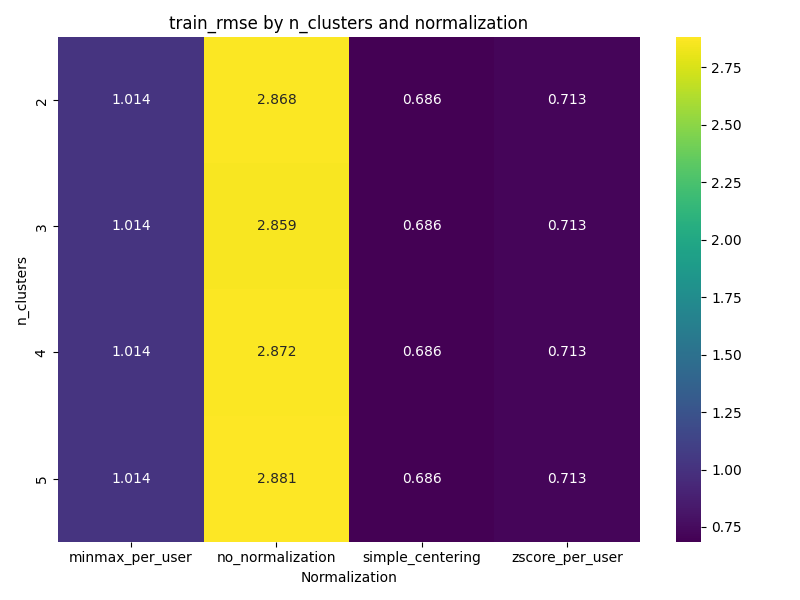
\includegraphics[width=0.8\textwidth]{../output/run_kmeans/images/train/rmse/heatmap_train_rmse.png}
  \caption{Heatmap - Train RMSE - Run K-Means}
  \label{fig:train_rmse_kmeans}
\end{figure}

In figura \ref{fig:train_rmse_kmeans} si può vedere l'heatmap del Train RMSE per le 4 differenti normalizzazioni. Si può confermare come simple\_centering si sia dimostrato il miglior metodo di normalizzazione per K-Means, con il metodo senza normalizzazione che offre le performance peggiori. Eccetto quest'ultima normalizzazione, nelle altre i valori di RMSE rimangono idenici al variare del numero di cluster.

\begin{table}[H]
  \centering
  \caption{Top 5 Configurazioni per Train MAE - Run K-Means}
  \resizebox{\textwidth}{!}{%
  \begin{tabular}{|l|c|c|c|c|c|c|c|c|}
  \hline
  \textbf{Rank} & \textbf{Normalization} & \textbf{Clusters} & \textbf{m} & \textbf{Method} & \textbf{Defuzz} & \textbf{Neighbor} & \textbf{Train MAE} & \textbf{Elapsed Sec}\\
  \hline
  1 & simple\_centering & 5 & 2.0 & kmeans & maximum & pearson & 0.509171 & 41.557193 \\
  2 & simple\_centering & 4 & 2.0 & kmeans & maximum & pearson & 0.509171 & 28.044528 \\
  3 & simple\_centering & 3 & 2.0 & kmeans & maximum & pearson & 0.509171 & 38.488144 \\
  4 & simple\_centering & 2 & 2.0 & kmeans & maximum & pearson & 0.509171 & 40.785123 \\
  5 & zscore\_per\_user & 2 & 2.0 & kmeans & maximum & pearson & 0.537192 & 43.493679 \\
  \hline
  \end{tabular}%
  }
\end{table}

Il pattern è identico al Train RMSE: simple\_centering ottiene lo stesso MAE (0.509171) per tutti i numeri di cluster. Questo conferma la mancanza di separazione significativa tra cluster. Andiamo ad osservarli.

\begin{figure}[H]
  \centering
  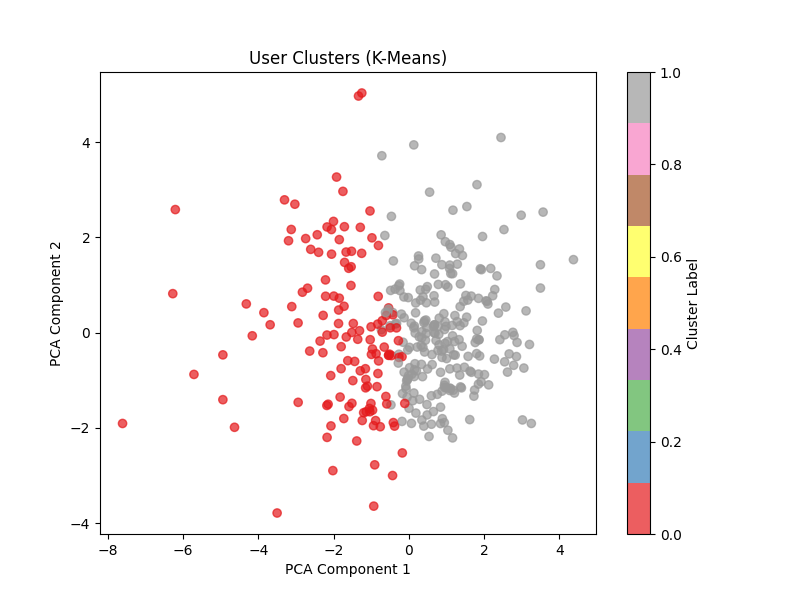
\includegraphics[width=0.5\textwidth]{../output/run_kmeans/images/normalization/simple_centering/hard_clusters/hard_clusters_pca_c2_m2.0_kmeans_maximum_pearson.png}
  \caption{2 Clusters - Run K-Means}
  \label{fig:2_clusters_kmeans}
\end{figure}
\begin{figure}[H]
  \centering
  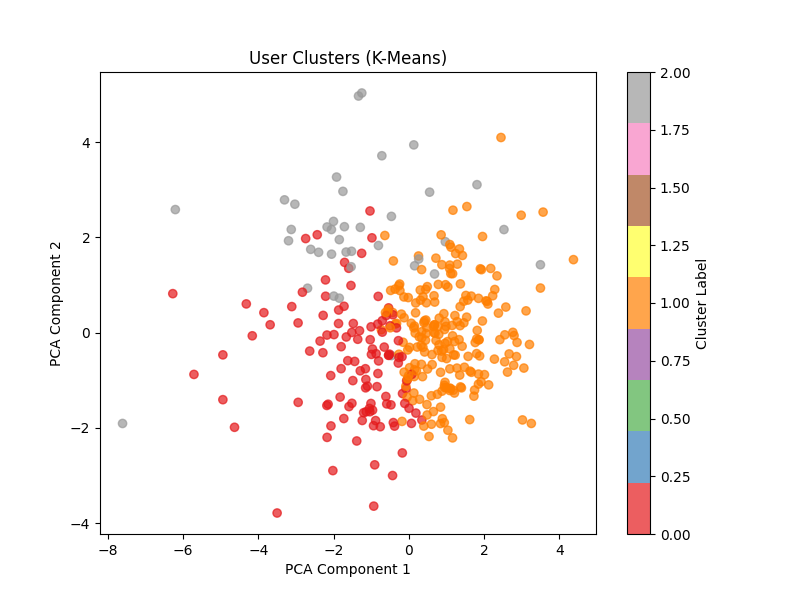
\includegraphics[width=0.5\textwidth]{../output/run_kmeans/images/normalization/simple_centering/hard_clusters/hard_clusters_pca_c3_m2.0_kmeans_maximum_pearson.png}
  \caption{3 Clusters - Run K-Means}
  \label{fig:3_clusters_kmeans}
\end{figure}
\begin{figure}[H]
  \centering
  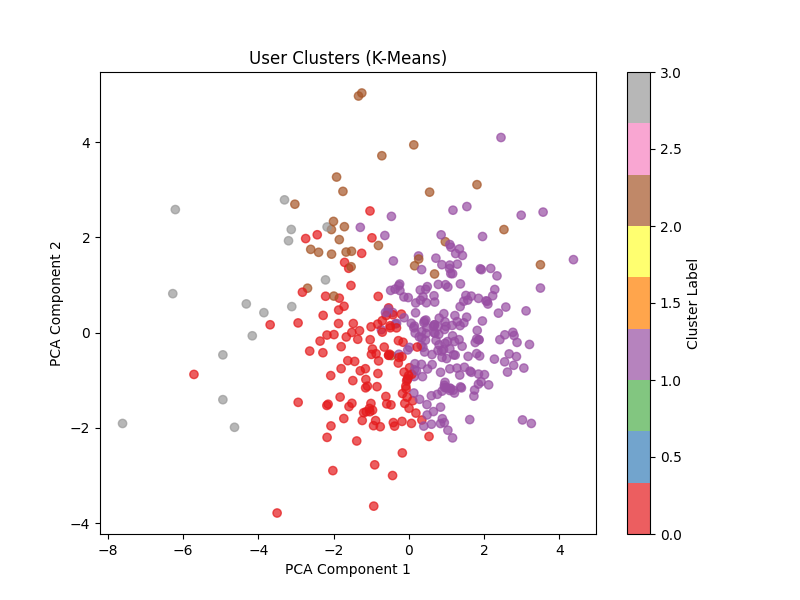
\includegraphics[width=0.5\textwidth]{../output/run_kmeans/images/normalization/simple_centering/hard_clusters/hard_clusters_pca_c4_m2.0_kmeans_maximum_pearson.png}
  \caption{4 Clusters - Run K-Means}
  \label{fig:4_clusters_kmeans}
\end{figure}
\begin{figure}[H]
  \centering
  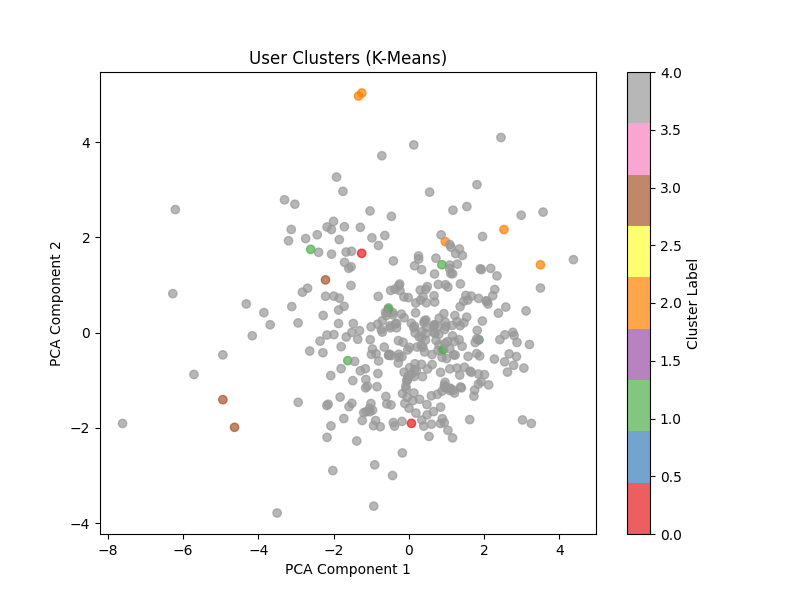
\includegraphics[width=0.5\textwidth]{../output/run_kmeans/images/normalization/simple_centering/hard_clusters/hard_clusters_pca_c5_m2.0_kmeans_maximum_pearson.png}
  \caption{5 Clusters - Run K-Means}
  \label{fig:5_clusters_kmeans}
\end{figure}

Come si può vedere dalle figure \ref{fig:2_clusters_kmeans}, \ref{fig:3_clusters_kmeans}, \ref{fig:4_clusters_kmeans} e \ref{fig:5_clusters_kmeans}, i dati sono molto densi e quindi il clustering non sta producendo separazioni significative, confermando quanto già osservato con le metriche.

\begin{table}[H]
  \centering
  \caption{Top 5 Configurazioni per Train Precision - Run K-Means}
  \resizebox{\textwidth}{!}{%
  \begin{tabular}{|l|c|c|c|c|c|c|c|c|}
  \hline
  \textbf{Rank} & \textbf{Normalization} & \textbf{Clusters} & \textbf{m} & \textbf{Method} & \textbf{Defuzz} & \textbf{Neighbor} & \textbf{Train Precision} & \textbf{Elapsed Sec}\\
  \hline
  1 & no\_normalization & 2 & 2.0 & kmeans & maximum & pearson & 0.588462 & 41.276888 \\
  2 & no\_normalization & 3 & 2.0 & kmeans & maximum & pearson & 0.588187 & 25.853554 \\
  3 & minmax\_per\_user & 3 & 2.0 & kmeans & maximum & pearson & 0.587637 & 21.230663 \\
  4 & minmax\_per\_user & 2 & 2.0 & kmeans & maximum & pearson & 0.587637 & 28.917084 \\
  5 & minmax\_per\_user & 5 & 2.0 & kmeans & maximum & pearson & 0.587637 & 14.610376 \\
  \hline
  \end{tabular}%
  }
\end{table}

Per le metriche di qualità delle raccomandazioni, no\_normalization e minmax\_per\_user dominano, a differenza delle metriche di errore. I valori di precision sono simili (~0.587-0.588) indipendentemente dal numero di cluster.

\begin{figure}[H]
  \centering
  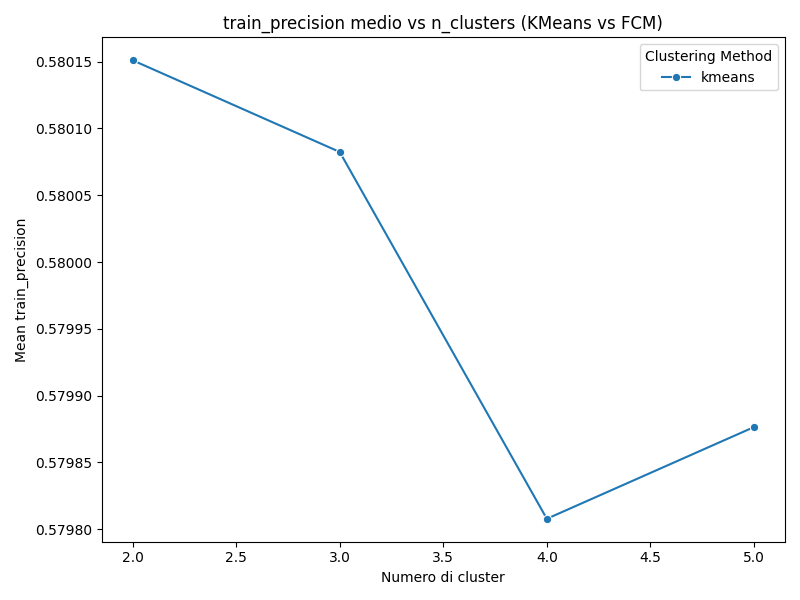
\includegraphics[width=0.8\textwidth]{../output/run_kmeans/images/train/precision/lineplot_nclusters_train_precision.png}
  \caption{Lineplot - Train Precision - Run K-Means}
  \label{fig:train_precision_kmeans}
\end{figure}

In figura \ref{fig:train_precision_kmeans} si può vedere il lineplot del Train Precision all'aumentare del numero di cluster. Si può notare come il valore di precision sia più alto con numero di cluster basso, sebbene con 5 fornisca una risalita rispetto a 4. 

\begin{table}[H]
  \centering
  \caption{Top 5 Configurazioni per Train Recall - Run K-Means}
  \resizebox{\textwidth}{!}{%
  \begin{tabular}{|l|c|c|c|c|c|c|c|c|}
  \hline
  \textbf{Rank} & \textbf{Normalization} & \textbf{Clusters} & \textbf{m} & \textbf{Method} & \textbf{Defuzz} & \textbf{Neighbor} & \textbf{Train Recall} & \textbf{Elapsed Sec}\\
  \hline
  1 & no\_normalization & 3 & 2.0 & kmeans & maximum & pearson & 0.138107 & 25.853554 \\
  2 & no\_normalization & 2 & 2.0 & kmeans & maximum & pearson & 0.138094 & 41.276888 \\
  3 & no\_normalization & 4 & 2.0 & kmeans & maximum & pearson & 0.137644 & 19.790054 \\
  4 & no\_normalization & 5 & 2.0 & kmeans & maximum & pearson & 0.137630 & 18.933092 \\
  5 & minmax\_per\_user & 5 & 2.0 & kmeans & maximum & pearson & 0.137605 & 14.610376 \\
  \hline
  \end{tabular}%
  }
\end{table}

I valori di recall sono molto bassi (~0.137-0.138). no\_normalization domina con valori leggermente decrescenti all'aumentare del numero di cluster, suggerendo un leggero overfitting, così come avveniva in precision.

\begin{table}[H]
  \centering
  \caption{Top 5 Configurazioni per Train Accuracy - Run K-Means}
  \resizebox{\textwidth}{!}{%
  \begin{tabular}{|l|c|c|c|c|c|c|c|c|}
  \hline
  \textbf{Rank} & \textbf{Normalization} & \textbf{Clusters} & \textbf{m} & \textbf{Method} & \textbf{Defuzz} & \textbf{Neighbor} & \textbf{Train Accuracy} & \textbf{Elapsed Sec}\\
  \hline
  1 & no\_normalization & 2 & 2.0 & kmeans & maximum & pearson & 0.588462 & 41.276888 \\
  2 & no\_normalization & 3 & 2.0 & kmeans & maximum & pearson & 0.588187 & 25.853554 \\
  3 & minmax\_per\_user & 3 & 2.0 & kmeans & maximum & pearson & 0.587637 & 21.230663 \\
  4 & minmax\_per\_user & 2 & 2.0 & kmeans & maximum & pearson & 0.587637 & 28.917084 \\
  5 & minmax\_per\_user & 5 & 2.0 & kmeans & maximum & pearson & 0.587637 & 14.610376 \\
  \hline
  \end{tabular}%
  }
\end{table}

I risultati sono identici al Train Precision, confermando che accuracy e precision coincidono.

\begin{figure}[H]
  \centering
  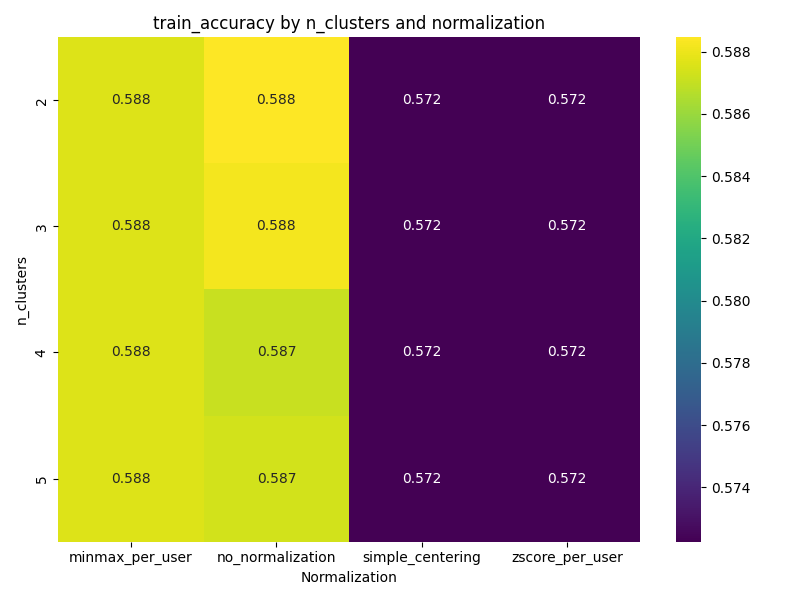
\includegraphics[width=0.8\textwidth]{../output/run_kmeans/images/train/accuracy/heatmap_train_accuracy.png}
  \caption{Heatmap - Train Accuracy - Run K-Means}
  \label{fig:train_accuracy_kmeans}
\end{figure}

In figura \ref{fig:train_accuracy_kmeans} si può osservare un risultato interessante: il clustering senza normalizzazione offre prestazioni simili alle tre tecniche di normalizzazione considerate, suggerendo che, almeno in questo contesto e con questi dati, le caratteristiche intrinseche dei dati sono già ben rappresentate senza la necessità di trasformazioni aggiuntive.

\begin{table}[H]
  \centering
  \caption{Top 5 Configurazioni per Train F1-Score - Run K-Means}
  \resizebox{\textwidth}{!}{%
  \begin{tabular}{|l|c|c|c|c|c|c|c|c|}
  \hline
  \textbf{Rank} & \textbf{Normalization} & \textbf{Clusters} & \textbf{m} & \textbf{Method} & \textbf{Defuzz} & \textbf{Neighbor} & \textbf{Train F1-Score} & \textbf{Elapsed Sec}\\
  \hline
  1 & no\_normalization & 2 & 2.0 & kmeans & maximum & pearson & 0.210876 & 41.276888 \\
  2 & no\_normalization & 3 & 2.0 & kmeans & maximum & pearson & 0.210854 & 25.853554 \\
  3 & minmax\_per\_user & 3 & 2.0 & kmeans & maximum & pearson & 0.210282 & 21.230663 \\
  4 & minmax\_per\_user & 2 & 2.0 & kmeans & maximum & pearson & 0.210282 & 28.917084 \\
  5 & minmax\_per\_user & 5 & 2.0 & kmeans & maximum & pearson & 0.210282 & 14.610376 \\
  \hline
  \end{tabular}%
  }
\end{table}

Gli F1-score sono bassi (~0.21) a causa dei valori di recall molto bassi. no\_normalization ottiene i migliori risultati, con valori leggermente decrescenti all'aumentare del numero di cluster.

\subsection{Test}

\begin{table}[H]
  \centering
  \caption{Top 5 Configurazioni per Test RMSE - Run K-Means}
  \resizebox{\textwidth}{!}{%
  \begin{tabular}{|l|c|c|c|c|c|c|c|c|}
  \hline
  \textbf{Rank} & \textbf{Normalization} & \textbf{Clusters} & \textbf{m} & \textbf{Method} & \textbf{Defuzz} & \textbf{Neighbor} & \textbf{Test RMSE} & \textbf{Elapsed Sec}\\
  \hline
  1 & simple\_centering & 2 & 2.0 & kmeans & maximum & pearson & 0.681716 & 40.785123 \\
  2 & simple\_centering & 3 & 2.0 & kmeans & maximum & pearson & 0.681716 & 38.488144 \\
  3 & simple\_centering & 4 & 2.0 & kmeans & maximum & pearson & 0.681716 & 28.044528 \\
  4 & simple\_centering & 5 & 2.0 & kmeans & maximum & pearson & 0.681716 & 41.557193 \\
  5 & minmax\_per\_user & 5 & 2.0 & kmeans & maximum & pearson & 0.699511 & 14.610376 \\
  \hline
  \end{tabular}%
  }
\end{table}

Anche nel test, simple\_centering ottiene lo stesso RMSE (0.681716) per tutti i numeri di cluster. Il Test RMSE è leggermente migliore del Train RMSE, indicando una buona generalizzazione.

\begin{figure}[H]
  \centering
  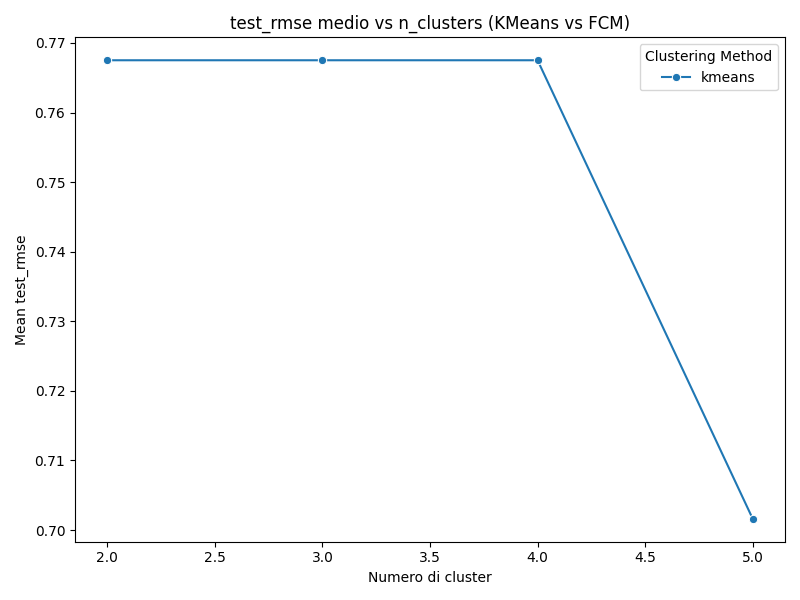
\includegraphics[width=0.8\textwidth]{../output/run_kmeans/images/test/rmse/lineplot_nclusters_test_rmse.png}
  \caption{Heatmap - Test RMSE - Run K-Means}
  \label{fig:test_rmse_kmeans}
\end{figure}

Dalla figura \ref{fig:test_rmse_kmeans} si può osservare che, in realtà, con 5 cluster, il Test RMSE peggiora notevolmente rispetto agli altri valori.


\begin{table}[H]
  \centering
  \caption{Top 5 Configurazioni per Test MAE - Run K-Means}
  \resizebox{\textwidth}{!}{%
  \begin{tabular}{|l|c|c|c|c|c|c|c|c|}
  \hline
  \textbf{Rank} & \textbf{Normalization} & \textbf{Clusters} & \textbf{m} & \textbf{Method} & \textbf{Defuzz} & \textbf{Neighbor} & \textbf{Test MAE} & \textbf{Elapsed Sec}\\
  \hline
  1 & zscore\_per\_user & 5 & 2.0 & kmeans & maximum & pearson & 0.540973 & 38.939321 \\
  2 & zscore\_per\_user & 4 & 2.0 & kmeans & maximum & pearson & 0.540973 & 45.033325 \\
  3 & zscore\_per\_user & 3 & 2.0 & kmeans & maximum & pearson & 0.540973 & 37.246547 \\
  4 & zscore\_per\_user & 2 & 2.0 & kmeans & maximum & pearson & 0.540973 & 43.493679 \\
  5 & simple\_centering & 2 & 2.0 & kmeans & maximum & pearson & 0.547638 & 40.785123 \\
  \hline
  \end{tabular}%
  }
\end{table}

A differenza delle altre metriche, zscore\_per\_user domina il Test MAE con lo stesso valore (0.540973) per tutti i numeri di cluster. Questo suggerisce una diversa sensibilità della metrica MAE alla normalizzazione.

\begin{figure}[H]
  \centering
  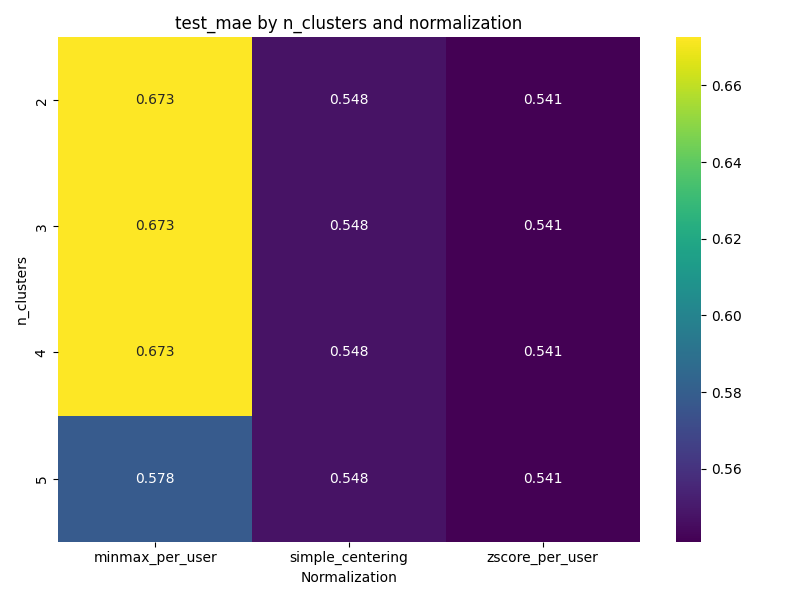
\includegraphics[width=0.8\textwidth]{../output/run_kmeans/images/test/mae/heatmap_test_mae.png}
  \caption{Heatmap - Test MAE - Run K-Means}
  \label{fig:test_mae_kmeans}
\end{figure}

In figura \ref{fig:test_mae_kmeans} possiamo confermare quanto emerso dalla tabella: zscore\_per\_user offre prestazioni migliori rispetto alle altre normalizzazioni.

\begin{table}[H]
  \centering
  \caption{Top 5 Configurazioni per Test Precision - Run K-Means}
  \resizebox{\textwidth}{!}{%
  \begin{tabular}{|l|c|c|c|c|c|c|c|c|}
  \hline
  \textbf{Rank} & \textbf{Normalization} & \textbf{Clusters} & \textbf{m} & \textbf{Method} & \textbf{Defuzz} & \textbf{Neighbor} & \textbf{Test Precision} & \textbf{Elapsed Sec}\\
  \hline
  1 & simple\_centering & 5 & 2.0 & kmeans & maximum & pearson & 0.605029 & 41.557193 \\
  2 & simple\_centering & 4 & 2.0 & kmeans & maximum & pearson & 0.605029 & 28.044528 \\
  3 & simple\_centering & 3 & 2.0 & kmeans & maximum & pearson & 0.605029 & 38.488144 \\
  4 & simple\_centering & 2 & 2.0 & kmeans & maximum & pearson & 0.605029 & 40.785123 \\
  5 & zscore\_per\_user & 2 & 2.0 & kmeans & maximum & pearson & 0.605029 & 43.493679 \\
  \hline
  \end{tabular}%
  }
\end{table}

A differenza del train, simple\_centering domina il Test Precision con lo stesso valore (0.605029) per tutti i numeri di cluster. Questo valore è identico al miglior risultato FCM, suggerendo performance simili.

\begin{table}[H]
  \centering
  \caption{Top 5 Configurazioni per Test Recall - Run K-Means}
  \resizebox{\textwidth}{!}{%
  \begin{tabular}{|l|c|c|c|c|c|c|c|c|}
  \hline
  \textbf{Rank} & \textbf{Normalization} & \textbf{Clusters} & \textbf{m} & \textbf{Method} & \textbf{Defuzz} & \textbf{Neighbor} & \textbf{Test Recall} & \textbf{Elapsed Sec}\\
  \hline
  1 & simple\_centering & 5 & 2.0 & kmeans & maximum & pearson & 0.511998 & 41.557193 \\
  2 & simple\_centering & 4 & 2.0 & kmeans & maximum & pearson & 0.511998 & 28.044528 \\
  3 & simple\_centering & 3 & 2.0 & kmeans & maximum & pearson & 0.511998 & 38.488144 \\
  4 & simple\_centering & 2 & 2.0 & kmeans & maximum & pearson & 0.511998 & 40.785123 \\
  5 & zscore\_per\_user & 2 & 2.0 & kmeans & maximum & pearson & 0.511835 & 43.493679 \\
  \hline
  \end{tabular}%
  }
\end{table}

Il pattern è identico al Test Precision. I valori di recall (~0.51) sono molto più alti rispetto al train (~0.14), identici a FCM. Questo suggerisce una migliore capacità di generalizzazione per entrambi gli algoritmi.

\begin{table}[H]
  \centering
  \caption{Top 5 Configurazioni per Test Accuracy - Run K-Means}
  \resizebox{\textwidth}{!}{%
  \begin{tabular}{|l|c|c|c|c|c|c|c|c|}
  \hline
  \textbf{Rank} & \textbf{Normalization} & \textbf{Clusters} & \textbf{m} & \textbf{Method} & \textbf{Defuzz} & \textbf{Neighbor} & \textbf{Test Accuracy} & \textbf{Elapsed Sec}\\
  \hline
  1 & simple\_centering & 5 & 2.0 & kmeans & maximum & pearson & 0.605029 & 41.557193 \\
  2 & simple\_centering & 4 & 2.0 & kmeans & maximum & pearson & 0.605029 & 28.044528 \\
  3 & simple\_centering & 3 & 2.0 & kmeans & maximum & pearson & 0.605029 & 38.488144 \\
  4 & simple\_centering & 2 & 2.0 & kmeans & maximum & pearson & 0.605029 & 40.785123 \\
  5 & zscore\_per\_user & 2 & 2.0 & kmeans & maximum & pearson & 0.605029 & 43.493679 \\
  \hline
  \end{tabular}%
  }
\end{table}

I risultati sono identici al Test Precision, confermando che accuracy e precision coincidono anche per K-Means nella fase di test. Questo pattern è consistente con FCM.

\begin{table}[H]
  \centering
  \caption{Top 5 Configurazioni per Test F1-Score - Run K-Means}
  \resizebox{\textwidth}{!}{%
  \begin{tabular}{|l|c|c|c|c|c|c|c|c|}
  \hline
  \textbf{Rank} & \textbf{Normalization} & \textbf{Clusters} & \textbf{m} & \textbf{Method} & \textbf{Defuzz} & \textbf{Neighbor} & \textbf{Test F1-Score} & \textbf{Elapsed Sec}\\
  \hline
  1 & simple\_centering & 5 & 2.0 & kmeans & maximum & pearson & 0.524162 & 41.557193 \\
  2 & simple\_centering & 4 & 2.0 & kmeans & maximum & pearson & 0.524162 & 28.044528 \\
  3 & simple\_centering & 3 & 2.0 & kmeans & maximum & pearson & 0.524162 & 38.488144 \\
  4 & simple\_centering & 2 & 2.0 & kmeans & maximum & pearson & 0.524162 & 40.785123 \\
  5 & zscore\_per\_user & 2 & 2.0 & kmeans & maximum & pearson & 0.524015 & 43.493679 \\
  \hline
  \end{tabular}%
  }
\end{table}

Gli F1-score (~0.52) sono significativamente più alti rispetto al train (~0.21) grazie ai valori di recall più elevati, identici a FCM. Il pattern di normalizzazione e cluster è identico alle altre metriche di test.

\subsection{Conclusioni K-Means}

I risultati della run K-Means rivelano pattern interessanti.

Per quanto riguarda le metriche RMSE e MAE, simple\_centering emerge come la normalizzazione dominante sia in fase di train che di test. I valori di RMSE (~0.68-0.69) e MAE (~0.51-0.55) indicano che il sistema commette errori medi di circa 0.7 stelle su una scala da 1 a 5 nel predire i rating degli utenti. Questo significa che se un utente ha dato 4 stelle a un film, il sistema potrebbe prevedere 3.3 o 4.7 stelle. Nel contesto pratico, questo livello di errore è accettabile per un sistema di raccomandazione, considerando che la scala di rating è soggettiva e che differenze di 0.5-1 stella sono spesso considerate normali tra utenti diversi.

La mancanza di variazione nei valori di errore al variare del numero di cluster (2-5) suggerisce che il clustering non sta producendo separazioni significative tra i profili utente. Questo fenomeno può essere interpretato positivamente: indica che gli utenti del dataset MovieLens 100k, dopo il filtraggio per densità, mostrano preferenze cinematografiche relativamente omogenee. In pratica, questo significa che la maggior parte degli utenti attivi (con almeno 150 rating) tende ad apprezzare film simili, rendendo difficile identificare cluster distinti di gusti cinematografici.

Le metriche di qualità rivelano una dicotomia interessante tra fase di train e test. In training, no\_normalization e minmax\_per\_user dominano con valori di precision e accuracy intorno al 58.8\%. Questo significa che il 58.8\% dei film raccomandati dal sistema sono effettivamente apprezzati dall'utente (rating $\geq$ 4.0). Tuttavia, i valori di recall molto bassi (~13.8\%) indicano che il sistema riesce a catturare solo una piccola frazione degli item che l'utente apprezza.

In fase di test, si osserva un miglioramento significativo: simple\_centering domina con precision/accuracy del 60.5\% e recall del 51.2\%. Questo miglioramento suggerisce che il sistema generalizza bene su nuovi dati, riuscendo a catturare una porzione maggiore delle preferenze dell'utente. Il fatto che il recall raddoppi quasi (da 13.8\% a 51.2\%) indica una migliore capacità di scoprire film che l'utente potrebbe apprezzare ma non ha ancora valutato.

\section{Run FCM}

Una volta eseguita la run con K-Means e analizzati i risultati, si è deciso di eseguire una run con FCM per capire se un algoritmo fuzzy può migliorare le prestazioni permettendo di catturare la sfumatura delle preferenze cinematografiche degli utenti.

\subsection{Train}

\begin{table}[H]
  \centering
  \caption{Top 5 Configurazioni per Train RMSE - Run FCM}
  \resizebox{\textwidth}{!}{%
  \begin{tabular}{|l|c|c|c|c|c|c|c|c|c|c|}
  \hline
  \textbf{Rank} & \textbf{Normalization} & \textbf{Clusters} & \textbf{m} & \textbf{Method} & \textbf{Defuzz} & \textbf{Neighbor} & \textbf{Train RMSE} & \textbf{Avg Max Membership} & \textbf{Avg Entropy} & \textbf{Elapsed Sec}\\
  \hline
  1 & simple\_centering & 2 & 1.2 & fcm & maximum & pearson & 0.685134 & 0.5 & 0.693147 & 39.334954 \\
  2 & simple\_centering & 2 & 1.2 & fcm & cog & pearson & 0.685134 & 0.5 & 0.693147 & 39.532738 \\
  3 & simple\_centering & 2 & 1.5 & fcm & maximum & pearson & 0.685134 & 0.5 & 0.693147 & 39.051460 \\
  4 & simple\_centering & 2 & 1.5 & fcm & cog & pearson & 0.685134 & 0.5 & 0.693147 & 39.617368 \\
  5 & simple\_centering & 2 & 1.8 & fcm & maximum & pearson & 0.685134 & 0.5 & 0.693147 & 39.740233 \\
  \hline
  \end{tabular}%
  }
\end{table}

Si osserva che tutte le configurazioni ottimali utilizzano simple\_centering con 2 cluster, indipendentemente dal valore di fuzziness (m) e dal metodo di defuzzificazione. I valori di Avg Max Membership (0.5) e Avg Entropy (0.693) sono identici per tutte le configurazioni, suggerendo una distribuzione uniforme delle membership.

\begin{figure}[H]
  \centering
  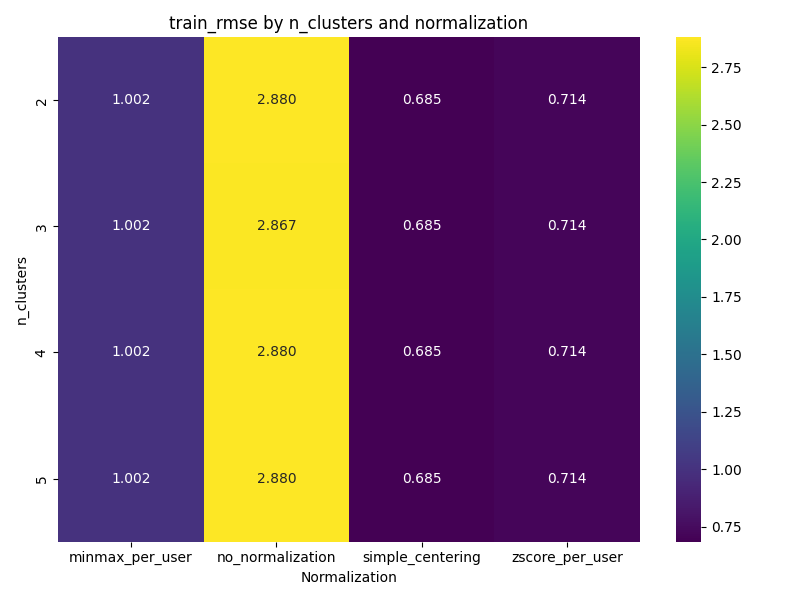
\includegraphics[width=0.8\textwidth]{../output/run_fcm/images/train/rmse/heatmap_train_rmse.png}
  \caption{Heatmap - Train RMSE - Run FCM}
  \label{fig:train_rmse_fcm}
\end{figure}

In figura \ref{fig:train_rmse_fcm} si può confermare come simple\_centering offre prestazioni migliori rispetto alle altre configurazioni.

\begin{table}[H]
  \centering
  \caption{Top 5 Configurazioni per Train MAE - Run FCM}
  \resizebox{\textwidth}{!}{%
  \begin{tabular}{|l|c|c|c|c|c|c|c|c|c|c|}
  \hline
  \textbf{Rank} & \textbf{Normalization} & \textbf{Clusters} & \textbf{m} & \textbf{Method} & \textbf{Defuzz} & \textbf{Neighbor} & \textbf{Train MAE} & \textbf{Avg Max Membership} & \textbf{Avg Entropy} & \textbf{Elapsed Sec}\\
  \hline
  1 & simple\_centering & 2 & 1.2 & fcm & maximum & pearson & 0.510734 & 0.5 & 0.693147 & 39.334954 \\
  2 & simple\_centering & 2 & 1.2 & fcm & cog & pearson & 0.510734 & 0.5 & 0.693147 & 39.532738 \\
  3 & simple\_centering & 2 & 1.5 & fcm & maximum & pearson & 0.510734 & 0.5 & 0.693147 & 39.051460 \\
  4 & simple\_centering & 2 & 1.5 & fcm & cog & pearson & 0.510734 & 0.5 & 0.693147 & 39.617368 \\
  5 & simple\_centering & 2 & 1.8 & fcm & maximum & pearson & 0.510734 & 0.5 & 0.693147 & 39.740233 \\
  \hline
  \end{tabular}%
  }
\end{table}

Il pattern è identico al Train RMSE: simple\_centering con 2 cluster domina, con valori identici di MAE, Avg Max Membership e Avg Entropy per tutte le configurazioni. Questo suggerisce che il numero di cluster ha un impatto maggiore dei parametri di fuzziness.

\begin{table}[H]
  \centering
  \caption{Top 5 Configurazioni per Train Precision - Run FCM}
  \resizebox{\textwidth}{!}{%
  \begin{tabular}{|l|c|c|c|c|c|c|c|c|c|c|}
  \hline
  \textbf{Rank} & \textbf{Normalization} & \textbf{Clusters} & \textbf{m} & \textbf{Method} & \textbf{Defuzz} & \textbf{Neighbor} & \textbf{Train Precision} & \textbf{Avg Max Membership} & \textbf{Avg Entropy} & \textbf{Elapsed Sec}\\
  \hline
  1 & no\_normalization & 3 & 1.2 & fcm & cog & pearson & 0.589011 & 0.446683 & 1.019679 & 43.236223 \\
  2 & no\_normalization & 2 & 1.2 & fcm & maximum & pearson & 0.588187 & 0.621032 & 0.645280 & 40.750197 \\
  3 & no\_normalization & 2 & 1.5 & fcm & maximum & pearson & 0.588187 & 0.5 & 0.693147 & 42.361609 \\
  4 & no\_normalization & 2 & 1.2 & fcm & cog & pearson & 0.588187 & 0.621032 & 0.645280 & 41.118601 \\
  5 & no\_normalization & 2 & 1.8 & fcm & maximum & pearson & 0.588187 & 0.5 & 0.693147 & 41.554277 \\
  \hline
  \end{tabular}%
  }
\end{table}

Per le metriche di qualità delle raccomandazioni, no\_normalization domina le classifiche. Si nota una correlazione tra Avg Max Membership e Avg Entropy: valori più alti di membership corrispondono a entropia più bassa, indicando cluster più definiti. I valori, inoltre, non sono più esattamente 0.5 e 0.693 come in K-Means, ma sono leggermente diversi, indicando che il clustering fuzzy produce cluster più sfumati.

\begin{figure}[H]
  \centering
  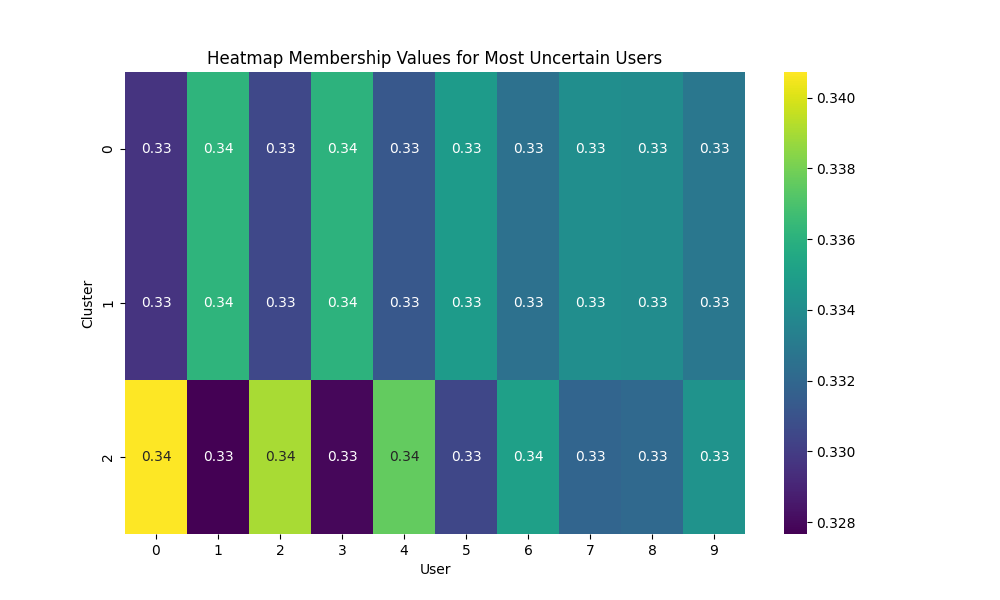
\includegraphics[width=0.8\textwidth]{../output/run_fcm/images/normalization/no_normalization/membership_heatmap/membership_heatmap_c3_m1.2_fcm_cog_pearson.png}
  \caption{Heatmap - Train Precision - Run FCM}
  \label{fig:train_precision_fcm}
\end{figure}

In figura \ref{fig:train_precision_fcm} si può confermare questa leggera sfumatura dei cluster.

\begin{table}[H]
  \centering
  \caption{Top 5 Configurazioni per Train Recall - Run FCM}
  \resizebox{\textwidth}{!}{%
  \begin{tabular}{|l|c|c|c|c|c|c|c|c|c|c|}
  \hline
  \textbf{Rank} & \textbf{Normalization} & \textbf{Clusters} & \textbf{m} & \textbf{Method} & \textbf{Defuzz} & \textbf{Neighbor} & \textbf{Train Recall} & \textbf{Avg Max Membership} & \textbf{Avg Entropy} & \textbf{Elapsed Sec}\\
  \hline
  1 & no\_normalization & 3 & 1.2 & fcm & cog & pearson & 0.138085 & 0.446683 & 1.019679 & 43.236223 \\
  2 & no\_normalization & 2 & 1.2 & fcm & maximum & pearson & 0.137792 & 0.621032 & 0.645280 & 40.750197 \\
  3 & no\_normalization & 2 & 1.5 & fcm & maximum & pearson & 0.137792 & 0.5 & 0.693147 & 42.361609 \\
  4 & no\_normalization & 2 & 1.2 & fcm & cog & pearson & 0.137792 & 0.621032 & 0.645280 & 41.118601 \\
  5 & no\_normalization & 2 & 1.8 & fcm & maximum & pearson & 0.137792 & 0.5 & 0.693147 & 41.554277 \\
  \hline
  \end{tabular}%
  }
\end{table}

I valori di recall sono molto bassi (~0.137-0.138), indicando che il sistema raccomanda solo una piccola frazione degli item apprezzati dall'utente. Il pattern di normalizzazione e cluster è identico al Train Precision.

\begin{table}[H]
  \centering
  \caption{Top 5 Configurazioni per Train Accuracy - Run FCM}
  \resizebox{\textwidth}{!}{%
  \begin{tabular}{|l|c|c|c|c|c|c|c|c|c|c|}
  \hline
  \textbf{Rank} & \textbf{Normalization} & \textbf{Clusters} & \textbf{m} & \textbf{Method} & \textbf{Defuzz} & \textbf{Neighbor} & \textbf{Train Accuracy} & \textbf{Avg Max Membership} & \textbf{Avg Entropy} & \textbf{Elapsed Sec}\\
  \hline
  1 & no\_normalization & 3 & 1.2 & fcm & cog & pearson & 0.589011 & 0.446683 & 1.019679 & 43.236223 \\
  2 & no\_normalization & 2 & 1.2 & fcm & maximum & pearson & 0.588187 & 0.621032 & 0.645280 & 40.750197 \\
  3 & no\_normalization & 2 & 1.5 & fcm & maximum & pearson & 0.588187 & 0.5 & 0.693147 & 42.361609 \\
  4 & no\_normalization & 2 & 1.2 & fcm & cog & pearson & 0.588187 & 0.621032 & 0.645280 & 41.118601 \\
  5 & no\_normalization & 2 & 1.8 & fcm & maximum & pearson & 0.588187 & 0.5 & 0.693147 & 41.554277 \\
  \hline
  \end{tabular}%
  }
\end{table}

I risultati sono identici al Train Precision, confermando che per questo dataset e configurazione, accuracy e precision coincidono. Questo suggerisce che il sistema non sta raccomandando item che l'utente non apprezza.

\begin{figure}[H]
  \centering
  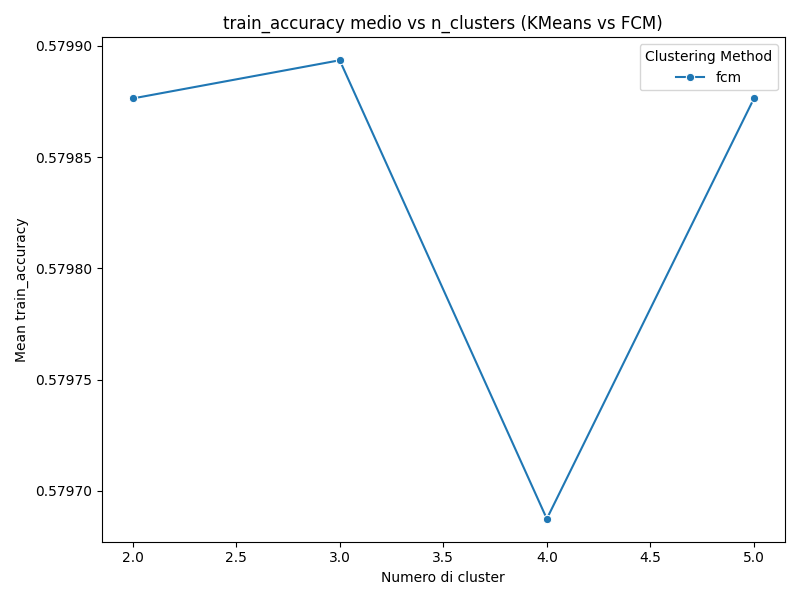
\includegraphics[width=0.8\textwidth]{../output/run_fcm/images/train/accuracy/lineplot_nclusters_train_accuracy.png.png}
  \caption{Lineplot - Train Accuracy - Run FCM}
  \label{fig:train_accuracy_fcm}
\end{figure}

In figura \ref{fig:train_accuracy_fcm} si può osservare come il Train Accuracy decresce intorno a 4 cluster, per poi aumentare di nuovo.

\begin{table}[H]
  \centering
  \caption{Top 5 Configurazioni per Train F1-Score - Run FCM}
  \resizebox{\textwidth}{!}{%
  \begin{tabular}{|l|c|c|c|c|c|c|c|c|c|c|}
  \hline
  \textbf{Rank} & \textbf{Normalization} & \textbf{Clusters} & \textbf{m} & \textbf{Method} & \textbf{Defuzz} & \textbf{Neighbor} & \textbf{Train F1-Score} & \textbf{Avg Max Membership} & \textbf{Avg Entropy} & \textbf{Elapsed Sec}\\
  \hline
  1 & no\_normalization & 3 & 1.2 & fcm & cog & pearson & 0.210995 & 0.446683 & 1.019679 & 43.236223 \\
  2 & no\_normalization & 2 & 1.2 & fcm & maximum & pearson & 0.210572 & 0.621032 & 0.645280 & 40.750197 \\
  3 & no\_normalization & 2 & 1.5 & fcm & maximum & pearson & 0.210572 & 0.5 & 0.693147 & 42.361609 \\
  4 & no\_normalization & 2 & 1.2 & fcm & cog & pearson & 0.210572 & 0.621032 & 0.645280 & 41.118601 \\
  5 & no\_normalization & 2 & 1.8 & fcm & maximum & pearson & 0.210572 & 0.5 & 0.693147 & 41.554277 \\
  \hline
  \end{tabular}%
  }
\end{table}

Gli F1-score sono bassi (~0.21) a causa dei valori di recall molto bassi. La configurazione con 3 cluster e cog defuzzification ottiene il miglior bilanciamento tra precision e recall.

\begin{table}[H]
  \centering
  \caption{Top 5 Configurazioni per Test RMSE - Run FCM}
  \resizebox{\textwidth}{!}{%
  \begin{tabular}{|l|c|c|c|c|c|c|c|c|c|c|}
  \hline
  \textbf{Rank} & \textbf{Normalization} & \textbf{Clusters} & \textbf{m} & \textbf{Method} & \textbf{Defuzz} & \textbf{Neighbor} & \textbf{Test RMSE} & \textbf{Avg Max Membership} & \textbf{Avg Entropy} & \textbf{Elapsed Sec}\\
  \hline
  1 & simple\_centering & 2 & 1.2 & fcm & maximum & pearson & 0.67889 & 0.5 & 0.693147 & 39.334954 \\
  2 & simple\_centering & 2 & 1.2 & fcm & cog & pearson & 0.67889 & 0.5 & 0.693147 & 39.532738 \\
  3 & simple\_centering & 2 & 1.5 & fcm & maximum & pearson & 0.67889 & 0.5 & 0.693147 & 39.051460 \\
  4 & simple\_centering & 2 & 1.5 & fcm & cog & pearson & 0.67889 & 0.5 & 0.693147 & 39.617368 \\
  5 & simple\_centering & 2 & 1.8 & fcm & maximum & pearson & 0.67889 & 0.5 & 0.693147 & 39.740233 \\
  \hline
  \end{tabular}%
  }
\end{table}

Il pattern è identico al Train RMSE: simple\_centering con 2 cluster domina. Il Test RMSE (0.6789) è leggermente migliore del Train RMSE (0.6851), suggerendo una buona generalizzazione.

\begin{table}[H]
  \centering
  \caption{Top 5 Configurazioni per Test MAE - Run FCM}
  \resizebox{\textwidth}{!}{%
  \begin{tabular}{|l|c|c|c|c|c|c|c|c|c|c|}
  \hline
  \textbf{Rank} & \textbf{Normalization} & \textbf{Clusters} & \textbf{m} & \textbf{Method} & \textbf{Defuzz} & \textbf{Neighbor} & \textbf{Test MAE} & \textbf{Avg Max Membership} & \textbf{Avg Entropy} & \textbf{Elapsed Sec}\\
  \hline
  1 & simple\_centering & 2 & 1.2 & fcm & maximum & pearson & 0.54478 & 0.5 & 0.693147 & 39.334954 \\
  2 & simple\_centering & 2 & 1.2 & fcm & cog & pearson & 0.54478 & 0.5 & 0.693147 & 39.532738 \\
  3 & simple\_centering & 2 & 1.5 & fcm & maximum & pearson & 0.54478 & 0.5 & 0.693147 & 39.051460 \\
  4 & simple\_centering & 2 & 1.5 & fcm & cog & pearson & 0.54478 & 0.5 & 0.693147 & 39.617368 \\
  5 & simple\_centering & 2 & 1.8 & fcm & maximum & pearson & 0.54478 & 0.5 & 0.693147 & 39.740233 \\
  \hline
  \end{tabular}%
  }
\end{table}

Stesso pattern del Test RMSE. Il Test MAE (0.5448) è leggermente peggiore del Train MAE (0.5107), ma la differenza è minima, indicando una buona stabilità del modello.

\begin{table}[H]
  \centering
  \caption{Top 5 Configurazioni per Test Precision - Run FCM}
  \resizebox{\textwidth}{!}{%
  \begin{tabular}{|l|c|c|c|c|c|c|c|c|c|c|}
  \hline
  \textbf{Rank} & \textbf{Normalization} & \textbf{Clusters} & \textbf{m} & \textbf{Method} & \textbf{Defuzz} & \textbf{Neighbor} & \textbf{Test Precision} & \textbf{Avg Max Membership} & \textbf{Avg Entropy} & \textbf{Elapsed Sec}\\
  \hline
  1 & zscore\_per\_user & 4 & 2.2 & fcm & maximum & pearson & 0.605029 & 0.25 & 1.386294 & 37.718682 \\
  2 & zscore\_per\_user & 4 & 2.2 & fcm & cog & pearson & 0.605029 & 0.25 & 1.386294 & 39.967926 \\
  3 & zscore\_per\_user & 4 & 2.5 & fcm & maximum & pearson & 0.605029 & 0.25 & 1.386294 & 40.161658 \\
  4 & zscore\_per\_user & 5 & 1.2 & fcm & maximum & pearson & 0.605029 & 0.2 & 1.609438 & 39.627358 \\
  5 & zscore\_per\_user & 5 & 1.5 & fcm & maximum & pearson & 0.605029 & 0.2 & 1.609438 & 50.886222 \\
  \hline
  \end{tabular}%
  }
\end{table}

A differenza del train, zscore\_per\_user domina con 4-5 cluster. I valori di Avg Max Membership sono più bassi (0.2-0.25) e Avg Entropy più alti (1.38-1.61), indicando cluster più fuzzy e sovrapposti.

\begin{figure}[H]
  \centering
  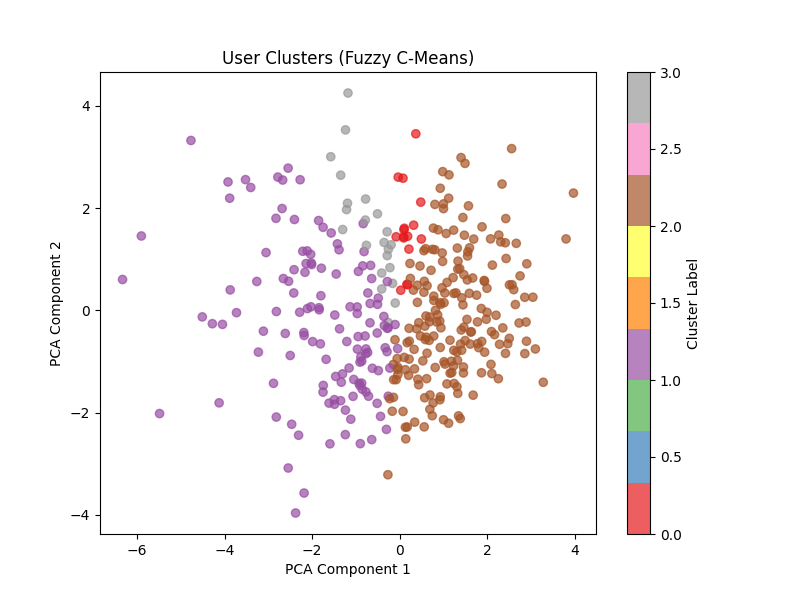
\includegraphics[width=0.8\textwidth]{../output/run_fcm/images/normalization/zscore_per_user/fuzzy_clusters/fuzzy_clusters_pca_c4_m2.2_fcm_maximum_pearson.png}
  \caption{Heatmap - Test Precision - Run FCM}
  \label{fig:test_precision_fcm}
\end{figure}

In figura \ref{fig:test_precision_fcm} riusciamo a osservare questa sfumatura dei cluster. Importante osservare come i cluster creati siano difficili da interpretare, in quanto non sono chiaramente separati.

\begin{table}[H]
  \centering
  \caption{Top 5 Configurazioni per Test Recall - Run FCM}
  \resizebox{\textwidth}{!}{%
  \begin{tabular}{|l|c|c|c|c|c|c|c|c|c|c|}
  \hline
  \textbf{Rank} & \textbf{Normalization} & \textbf{Clusters} & \textbf{m} & \textbf{Method} & \textbf{Defuzz} & \textbf{Neighbor} & \textbf{Test Recall} & \textbf{Avg Max Membership} & \textbf{Avg Entropy} & \textbf{Elapsed Sec}\\
  \hline
  1 & zscore\_per\_user & 4 & 2.2 & fcm & maximum & pearson & 0.511738 & 0.25 & 1.386294 & 37.718682 \\
  2 & zscore\_per\_user & 4 & 2.2 & fcm & cog & pearson & 0.511738 & 0.25 & 1.386294 & 39.967926 \\
  3 & zscore\_per\_user & 4 & 2.5 & fcm & maximum & pearson & 0.511738 & 0.25 & 1.386294 & 40.161658 \\
  4 & zscore\_per\_user & 5 & 1.2 & fcm & maximum & pearson & 0.511738 & 0.2 & 1.609438 & 39.627358 \\
  5 & zscore\_per\_user & 5 & 1.5 & fcm & maximum & pearson & 0.511738 & 0.2 & 1.609438 & 50.886222 \\
  \hline
  \end{tabular}%
  }
\end{table}

Il pattern è identico al Test Precision. I valori di recall (~0.51) sono molto più alti rispetto al train (~0.14), suggerendo una migliore capacità di catturare le preferenze dell'utente nel test set.

\begin{table}[H]
  \centering
  \caption{Top 5 Configurazioni per Test Accuracy - Run FCM}
  \resizebox{\textwidth}{!}{%
  \begin{tabular}{|l|c|c|c|c|c|c|c|c|c|c|}
  \hline
  \textbf{Rank} & \textbf{Normalization} & \textbf{Clusters} & \textbf{m} & \textbf{Method} & \textbf{Defuzz} & \textbf{Neighbor} & \textbf{Test Accuracy} & \textbf{Avg Max Membership} & \textbf{Avg Entropy} & \textbf{Elapsed Sec}\\
  \hline
  1 & zscore\_per\_user & 4 & 2.2 & fcm & maximum & pearson & 0.605029 & 0.25 & 1.386294 & 37.718682 \\
  2 & zscore\_per\_user & 4 & 2.2 & fcm & cog & pearson & 0.605029 & 0.25 & 1.386294 & 39.967926 \\
  3 & zscore\_per\_user & 4 & 2.5 & fcm & maximum & pearson & 0.605029 & 0.25 & 1.386294 & 40.161658 \\
  4 & zscore\_per\_user & 5 & 1.2 & fcm & maximum & pearson & 0.605029 & 0.2 & 1.609438 & 39.627358 \\
  5 & zscore\_per\_user & 5 & 1.5 & fcm & maximum & pearson & 0.605029 & 0.2 & 1.609438 & 50.886222 \\
  \hline
  \end{tabular}%
  }
\end{table}

I risultati sono identici al Test Precision, confermando che accuracy e precision coincidono anche nella fase di test. Questo pattern è consistente tra train e test.

\begin{table}[H]
  \centering
  \caption{Top 5 Configurazioni per Test F1-Score - Run FCM}
  \resizebox{\textwidth}{!}{%
  \begin{tabular}{|l|c|c|c|c|c|c|c|c|c|c|}
  \hline
  \textbf{Rank} & \textbf{Normalization} & \textbf{Clusters} & \textbf{m} & \textbf{Method} & \textbf{Defuzz} & \textbf{Neighbor} & \textbf{Test F1-Score} & \textbf{Avg Max Membership} & \textbf{Avg Entropy} & \textbf{Elapsed Sec}\\
  \hline
  1 & zscore\_per\_user & 4 & 2.2 & fcm & maximum & pearson & 0.52395 & 0.25 & 1.386294 & 37.718682 \\
  2 & zscore\_per\_user & 4 & 2.2 & fcm & cog & pearson & 0.52395 & 0.25 & 1.386294 & 39.967926 \\
  3 & zscore\_per\_user & 4 & 2.5 & fcm & maximum & pearson & 0.52395 & 0.25 & 1.386294 & 40.161658 \\
  4 & zscore\_per\_user & 5 & 1.2 & fcm & maximum & pearson & 0.52395 & 0.2 & 1.609438 & 39.627358 \\
  5 & zscore\_per\_user & 5 & 1.5 & fcm & maximum & pearson & 0.52395 & 0.2 & 1.609438 & 50.886222 \\
  \hline
  \end{tabular}%
  }
\end{table}

Gli F1-score (~0.52) sono significativamente più alti rispetto al train (~0.21) grazie ai valori di recall più elevati. Il pattern di normalizzazione e cluster è identico alle altre metriche di test.

\subsection{Conclusioni FCM}

I risultati della run FCM rivelano pattern interessanti che differiscono da quelli osservati con K-Means, evidenziando i vantaggi del clustering fuzzy nel contesto dei sistemi di raccomandazione cinematografici.

Per le metriche RMSE e MAE, FCM mostra performance simili a quelle offere da K-Means. Il Test RMSE di FCM (0.6789) è leggermente inferiore a quello di K-Means (0.6817), mentre il Test MAE di FCM (0.5448) è leggermente superiore a quello di K-Means (0.5409). Queste differenze risultano minime e dunque non sono significative.

Come per K-Means, simple\_centering domina le metriche di errore con 2 cluster, ma a differenza del clustering hard, FCM mostra valori di Avg Max Membership e Avg Entropy che variano leggermente tra le configurazioni, indicando una maggiore flessibilità nella rappresentazione delle preferenze.

Per le metriche di qualità delle raccomandazioni, FCM mostra performance identiche a K-Means, indicando che l'introduzione del clustering fuzzy non ha portato a miglioramenti significativi. In tabella \ref{tab:fcm_vs_kmeans} si può osservare un confronto tra le due tecniche.

\begin{table}[H]
  \centering
  \caption{Confronto Performance FCM vs K-Means}
  \label{tab:fcm_vs_kmeans}
  \begin{tabular}{|l|c|c|c|c|}
  \hline
  \textbf{Metrica} & \textbf{FCM Train} & \textbf{K-Means Train} & \textbf{FCM Test} & \textbf{K-Means Test} \\
  \hline
  RMSE & 0.6851 & 0.6864 & 0.6789 & 0.6817 \\
  MAE & 0.5107 & 0.5092 & 0.5448 & 0.5409 \\
  Precision & 58.9\% & 58.8\% & 60.5\% & 60.5\% \\
  Recall & 13.8\% & 13.8\% & 51.2\% & 51.2\% \\
  F1-Score & 21.1\% & 21.1\% & 52.4\% & 52.4\% \\
  \hline
  \end{tabular}
\end{table}


\appendix
\chapter{Appendice A: Risultati delle Run}
\label{chap:app1}

\section{Run Sample}

\subsection{Top 5 per Train RMSE - Run Sample}
\begin{table}[h]
    \centering
    \caption{Top 5 Configurazioni per Train RMSE - Run Sample}
    \begin{tabular}{|l|c|c|c|c|c|c|c|}
    \hline
    \textbf{Rank} & \textbf{Normalization} & \textbf{Clusters} & \textbf{m} & \textbf{Method} & \textbf{Defuzz} & \textbf{Neighbor} & \textbf{Train RMSE} \\
    \hline
    1 & simple\_centering & 8 & 1.5 & FCM & COG & Pearson & 3.870 \\
    2 & minmax\_per\_user & 8 & 1.5 & FCM & COG & Pearson & 3.950 \\
    3 & no\_normalization & 8 & 1.5 & FCM & COG & Pearson & 3.950 \\
    4 & zscore\_per\_user & 8 & 1.5 & FCM & COG & Pearson & 3.950 \\
    5 & simple\_centering & 8 & 2.0 & K-Means & COG & Pearson & 3.989 \\
    \hline
    \end{tabular}
    \end{table}

\subsection{Top 5 per Train MAE - Run Sample}
\begin{table}[h]
    \centering
    \caption{Top 5 Configurazioni per Train MAE - Run Sample}
    \begin{tabular}{|l|c|c|c|c|c|c|c|}
    \hline
    \textbf{Rank} & \textbf{Normalization} & \textbf{Clusters} & \textbf{m} & \textbf{Method} & \textbf{Defuzz} & \textbf{Neighbor} & \textbf{Train MAE} \\
    \hline
    1 & simple\_centering & 8 & 1.5 & FCM & COG & Pearson & 3.786 \\
    2 & minmax\_per\_user & 8 & 1.5 & FCM & COG & Pearson & 3.866 \\
    3 & no\_normalization & 8 & 1.5 & FCM & COG & Pearson & 3.866 \\
    4 & zscore\_per\_user & 8 & 1.5 & FCM & COG & Pearson & 3.866 \\
    5 & simple\_centering & 8 & 2.0 & K-Means & COG & Pearson & 3.898 \\
    \hline
    \end{tabular}
    \end{table}

\subsection{Top 5 per Test RMSE - Run Sample}
\begin{table}[h]
    \centering
    \caption{Top 5 Configurazioni per Test RMSE - Run Sample}
    \begin{tabular}{|l|c|c|c|c|c|c|c|}
    \hline
    \textbf{Rank} & \textbf{Normalization} & \textbf{Clusters} & \textbf{m} & \textbf{Method} & \textbf{Defuzz} & \textbf{Neighbor} & \textbf{Test RMSE} \\
    \hline
    1 & minmax\_per\_user & 8 & 1.5 & FCM & COG & Pearson & 3.816 \\
    2 & zscore\_per\_user & 8 & 1.5 & FCM & COG & Pearson & 3.816 \\
    3 & no\_normalization & 8 & 1.5 & FCM & COG & Pearson & 3.816 \\
    4 & no\_normalization & 4 & 1.5 & K-Means & COG & None & 3.816 \\
    5 & minmax\_per\_user & 4 & 2.0 & K-Means & Maximum & None & 3.816 \\
    \hline
    \end{tabular}
    \end{table}

\subsection{Top 5 per Test MAE - Run Sample}
\begin{table}[h]
    \centering
    \caption{Top 5 Configurazioni per Test MAE - Run Sample}
    \begin{tabular}{|l|c|c|c|c|c|c|c|}
    \hline
    \textbf{Rank} & \textbf{Normalization} & \textbf{Clusters} & \textbf{m} & \textbf{Method} & \textbf{Defuzz} & \textbf{Neighbor} & \textbf{Test MAE} \\
    \hline
    1 & zscore\_per\_user & 4 & 1.5 & K-Means & Maximum & None & 3.704 \\
    2 & minmax\_per\_user & 4 & 2.5 & K-Means & Maximum & None & 3.704 \\
    3 & zscore\_per\_user & 4 & 2.0 & K-Means & COG & None & 3.704 \\
    4 & zscore\_per\_user & 4 & 2.5 & K-Means & Maximum & None & 3.704 \\
    5 & no\_normalization & 4 & 2.0 & K-Means & Maximum & None & 3.704 \\
    \hline
    \end{tabular}
    \end{table}

\section{Run FCM Deep Dive}

\subsection{Top 5 per Train RMSE - Run FCM Deep Dive}
\begin{table}[h]
    \centering
    \caption{Top 5 Configurazioni per Train RMSE - Run FCM Deep Dive}
    \begin{tabular}{|l|c|c|c|c|c|c|c|}
    \hline
    \textbf{Rank} & \textbf{Normalization} & \textbf{Clusters} & \textbf{m} & \textbf{Method} & \textbf{Defuzz} & \textbf{Neighbor} & \textbf{Train RMSE} \\
    \hline
    1 & simple\_centering & 12 & 2.2 & FCM & COG & Pearson & 0.684 \\
    2 & simple\_centering & 8 & 1.8 & FCM & Maximum & Pearson & 0.691 \\
    3 & simple\_centering & 12 & 2.0 & FCM & COG & Pearson & 0.695 \\
    4 & simple\_centering & 6 & 1.5 & FCM & Maximum & Pearson & 0.696 \\
    5 & simple\_centering & 10 & 1.8 & FCM & Maximum & Pearson & 0.696 \\
    \hline
    \end{tabular}
    \end{table}

\subsection{Top 5 per Train MAE - Run FCM Deep Dive}
\begin{table}[h]
    \centering
    \caption{Top 5 Configurazioni per Train MAE - Run FCM Deep Dive}
    \begin{tabular}{|l|c|c|c|c|c|c|c|}
    \hline
    \textbf{Rank} & \textbf{Normalization} & \textbf{Clusters} & \textbf{m} & \textbf{Method} & \textbf{Defuzz} & \textbf{Neighbor} & \textbf{Train MAE} \\
    \hline
    1 & simple\_centering & 12 & 2.2 & FCM & COG & Pearson & 0.538 \\
    2 & simple\_centering & 12 & 2.0 & FCM & COG & Pearson & 0.546 \\
    3 & simple\_centering & 8 & 1.8 & FCM & Maximum & Pearson & 0.548 \\
    4 & simple\_centering & 12 & 2.2 & FCM & Maximum & Pearson & 0.549 \\
    5 & simple\_centering & 12 & 1.8 & FCM & Maximum & Pearson & 0.550 \\
    \hline
    \end{tabular}
    \end{table}

\subsection{Top 5 per Test RMSE - Run FCM Deep Dive}
\begin{table}[h]
    \centering
    \caption{Top 5 Configurazioni per Test RMSE - Run FCM Deep Dive}
    \begin{tabular}{|l|c|c|c|c|c|c|c|}
    \hline
    \textbf{Rank} & \textbf{Normalization} & \textbf{Clusters} & \textbf{m} & \textbf{Method} & \textbf{Defuzz} & \textbf{Neighbor} & \textbf{Test RMSE} \\
    \hline
    1 & simple\_centering & 12 & 2.0 & FCM & Maximum & Pearson & 0.594 \\
    2 & simple\_centering & 6 & 2.2 & FCM & Maximum & Pearson & 0.595 \\
    3 & simple\_centering & 12 & 2.2 & FCM & Maximum & Pearson & 0.598 \\
    4 & simple\_centering & 10 & 1.5 & FCM & Maximum & Pearson & 0.598 \\
    5 & simple\_centering & 12 & 1.8 & FCM & COG & Pearson & 0.600 \\
    \hline
    \end{tabular}
    \end{table}

\subsection{Top 5 per Test MAE - Run FCM Deep Dive}
\begin{table}[h]
    \centering
    \caption{Top 5 Configurazioni per Test MAE - Run FCM Deep Dive}
    \begin{tabular}{|l|c|c|c|c|c|c|c|}
    \hline
    \textbf{Rank} & \textbf{Normalization} & \textbf{Clusters} & \textbf{m} & \textbf{Method} & \textbf{Defuzz} & \textbf{Neighbor} & \textbf{Test MAE} \\
    \hline
    1 & simple\_centering & 6 & 2.2 & FCM & Maximum & Pearson & 0.468 \\
    2 & simple\_centering & 12 & 2.0 & FCM & Maximum & Pearson & 0.468 \\
    3 & simple\_centering & 12 & 2.2 & FCM & Maximum & Pearson & 0.470 \\
    4 & simple\_centering & 10 & 1.5 & FCM & Maximum & Pearson & 0.471 \\
    5 & simple\_centering & 12 & 1.8 & FCM & COG & Pearson & 0.471 \\
    \hline
    \end{tabular}
    \end{table}

\section{Run K-Means}

\subsection{Top 5 per Train RMSE - Run K-Means}
\begin{table}[h]
    \centering
    \caption{Top 5 Configurazioni per Train RMSE - Run K-Means}
    \begin{tabular}{|l|c|c|c|c|c|c|c|}
    \hline
    \textbf{Rank} & \textbf{Normalization} & \textbf{Clusters} & \textbf{m} & \textbf{Method} & \textbf{Defuzz} & \textbf{Neighbor} & \textbf{Train RMSE} \\
    \hline
    1 & simple\_centering & 4 & 1.5 & K-Means & Maximum & Pearson & 0.680 \\
    2 & simple\_centering & 4 & 1.5 & K-Means & COG & Pearson & 0.680 \\
    3 & simple\_centering & 4 & 2.0 & K-Means & COG & Pearson & 0.680 \\
    4 & simple\_centering & 4 & 2.0 & K-Means & Maximum & Pearson & 0.680 \\
    5 & simple\_centering & 4 & 2.5 & K-Means & COG & Pearson & 0.680 \\
    \hline
    \end{tabular}
    \end{table}

\subsection{Top 5 per Train MAE - Run K-Means}
\begin{table}[h]
    \centering
    \caption{Top 5 Configurazioni per Train MAE - Run K-Means}
    \begin{tabular}{|l|c|c|c|c|c|c|c|}
    \hline
    \textbf{Rank} & \textbf{Normalization} & \textbf{Clusters} & \textbf{m} & \textbf{Method} & \textbf{Defuzz} & \textbf{Neighbor} & \textbf{Train MAE} \\
    \hline
    1 & simple\_centering & 4 & 1.5 & K-Means & Maximum & Pearson & 0.531 \\
    2 & simple\_centering & 4 & 1.5 & K-Means & COG & Pearson & 0.531 \\
    3 & simple\_centering & 4 & 2.0 & K-Means & COG & Pearson & 0.531 \\
    4 & simple\_centering & 4 & 2.0 & K-Means & Maximum & Pearson & 0.531 \\
    5 & simple\_centering & 4 & 2.5 & K-Means & COG & Pearson & 0.531 \\
    \hline
    \end{tabular}
    \end{table}

\subsection{Top 5 per Test RMSE - Run K-Means}
\begin{table}[h]
    \centering
    \caption{Top 5 Configurazioni per Test RMSE - Run K-Means}
    \begin{tabular}{|l|c|c|c|c|c|c|c|}
    \hline
    \textbf{Rank} & \textbf{Normalization} & \textbf{Clusters} & \textbf{m} & \textbf{Method} & \textbf{Defuzz} & \textbf{Neighbor} & \textbf{Test RMSE} \\
    \hline
    1 & simple\_centering & 15 & 1.5 & K-Means & Maximum & Pearson & 0.597 \\
    2 & simple\_centering & 15 & 1.5 & K-Means & COG & Pearson & 0.597 \\
    3 & simple\_centering & 15 & 2.0 & K-Means & COG & Pearson & 0.597 \\
    4 & simple\_centering & 15 & 2.0 & K-Means & Maximum & Pearson & 0.597 \\
    5 & simple\_centering & 15 & 2.5 & K-Means & Maximum & Pearson & 0.597 \\
    \hline
    \end{tabular}
    \end{table}

\subsection{Top 5 per Test MAE - Run K-Means}
\begin{table}[h]
    \centering
    \caption{Top 5 Configurazioni per Test MAE - Run K-Means}
    \begin{tabular}{|l|c|c|c|c|c|c|c|}
    \hline
    \textbf{Rank} & \textbf{Normalization} & \textbf{Clusters} & \textbf{m} & \textbf{Method} & \textbf{Defuzz} & \textbf{Neighbor} & \textbf{Test MAE} \\
    \hline
    1 & simple\_centering & 15 & 1.5 & K-Means & Maximum & Pearson & 0.465 \\
    2 & simple\_centering & 15 & 1.5 & K-Means & COG & Pearson & 0.465 \\
    3 & simple\_centering & 15 & 2.0 & K-Means & COG & Pearson & 0.465 \\
    4 & simple\_centering & 15 & 2.0 & K-Means & Maximum & Pearson & 0.465 \\
    5 & simple\_centering & 15 & 2.5 & K-Means & Maximum & Pearson & 0.465 \\
    \hline
    \end{tabular}
    \end{table}


\backmatter
\sloppy 
\printbibliography[heading=bibintoc, title=Bibliografia]

\newpage 


\end{document} 
